\documentclass[10pt]{article}
\usepackage[T1]{fontenc}
\usepackage[utf8]{inputenc}
%\usepackage[latin1]{inputenc}
\DeclareUnicodeCharacter{00A0}{ }
% \usepackage{lmodern}
%\usepackage[adobe-utopia,uppercase=upright,greeklowercase=upright]{mathdesign}
\usepackage[adobe-utopia]{mathdesign}
%\usepackage{minionpro}
% \usepackage{pifont}
% \usepackage{amssymb}
\usepackage{amsmath}
\usepackage[francais]{babel}
% \usepackage[francais]{varioref}
\usepackage[dvips]{graphicx}
\usepackage{here}
\usepackage{framed}
\usepackage[normalem]{ulem}
\usepackage{fancyhdr}
\usepackage{titlesec}
\usepackage{vmargin}
\usepackage{longtable}

\usepackage{amsmath}

\usepackage{ifthen}
%\usepackage[•]{caption}

%\usepackage{epsfig}
\usepackage{subfig}

\usepackage{multirow}
\usepackage{multicol} % Portions de texte en colonnes
\usepackage{flafter}%floatants après la référence



\usepackage{color}
\usepackage{colortbl}


\definecolor{gris25}{gray}{0.75}
\definecolor{bleu}{RGB}{18,33,98}
\definecolor{bleuf}{RGB}{42,94,171}
\definecolor{bleuc}{RGB}{231,239,247}
\definecolor{rougef}{RGB}{185,18,27}
\definecolor{rougec}{RGB}{255,230,231}
\definecolor{vertf}{RGB}{103,126,82}
\definecolor{vertc}{RGB}{220,255,191}
\definecolor{violetf}{RGB}{112,48,160}
\definecolor{violetc}{RGB}{230,224,236}
\definecolor{jaunec}{RGB}{220,255,191}

\newenvironment{sci}[1][\hsize]%
{%
    \def\FrameCommand%
    {%
%\rotatebox{90}{\textit{\textsf{Scilab}}
\includegraphics[height=.8cm]{png/logo_scilab}} 
\rotatebox{90}{
\includegraphics[height=.6cm]{png/logo_scilab}} 
        {\color{violetf}\vrule width 3pt}%
        \hspace{0pt}%must no space.
        \fboxsep=\FrameSep\colorbox{violetc}%
    }%
    \MakeFramed{\hsize #1 \advance\hsize-\width\FrameRestore}%
}%
{\endMakeFramed}%

\newenvironment{pseudo}[1][\hsize]%
{%
    \def\FrameCommand%
    {%
\rotatebox{90}{\textit{\textsf{Pseudo Code}}} 
        {\color{violetf}\vrule width 3pt}%
        \hspace{0pt}%must no space.
        \fboxsep=\FrameSep\colorbox{violetc}%
    }%
    \MakeFramed{\hsize #1 \advance\hsize-\width\FrameRestore}%
}%
{\endMakeFramed}%

\newenvironment{py}[1][\hsize]%
{%
    \def\FrameCommand%
    {%
%\rotatebox{90}{\textit{\textsf{Python}}} 
\rotatebox{90}{
\includegraphics[height=.6cm]{png/logo_python}} 
        {\color{violetf}\vrule width 3pt}%
        \hspace{0pt}%must no space.
        \fboxsep=\FrameSep\colorbox{violetc}%
    }%
    \MakeFramed{\hsize #1 \advance\hsize-\width\FrameRestore}%
}%
{\endMakeFramed}%


\newenvironment{term}[1][\hsize]%
{%
    \def\FrameCommand%
    {%
\rotatebox{90}{\textit{\textsf{Terminal}}} 
        {\color{violetf}\vrule width 3pt}%
        \hspace{0pt}%must no space.
        \fboxsep=\FrameSep\colorbox{violetc}%
    }%
    \MakeFramed{\hsize #1 \advance\hsize-\width\FrameRestore}%
}%
{\endMakeFramed}%


\newenvironment{rem}[1][\hsize]%
{%
    \def\FrameCommand
    {%
\rotatebox{90}{\textit{\textsf{Remarque}}} 
        {\color{bleuf}\vrule width 3pt}%
        \hspace{0pt}%must no space.
        \fboxsep=\FrameSep\colorbox{bleuc}%
    }%
    \MakeFramed{\hsize#1\advance\hsize-\width\FrameRestore}%
}%
{\endMakeFramed}%


\newenvironment{savoir}[1][\hsize]%
{%
    \def\FrameCommand
    {%
\rotatebox{90}{\textit{\textsf{Savoir}}} 
        {\color{bleuf}\vrule width 3pt}%
        \hspace{0pt}%must no space.
        \fboxsep=\FrameSep\colorbox{bleuc}%
    }%
    \MakeFramed{\hsize#1\advance\hsize-\width\FrameRestore}%
}%
{\endMakeFramed}%

\newenvironment{objectif}[1][\hsize]%
{%
    \def\FrameCommand
    {%
\rotatebox{90}{\textit{\textsf{Objectif}}} 
        {\color{rougef}\vrule width 3pt}%
        \hspace{0pt}%must no space.
        \fboxsep=\FrameSep\colorbox{rougec}%
    }%
    \MakeFramed{\hsize#1\advance\hsize-\width\FrameRestore}%
}%
{\endMakeFramed}%

\newenvironment{prob}[1][\hsize]%
{%
    \def\FrameCommand%
    {%
\rotatebox{90}{\textit{\textsf{ Problématique}}} 
        {\color{rougef}\vrule width 3pt}%
        \hspace{0pt}%must no space.
        \fboxsep=\FrameSep\colorbox{rougec}%
    }%
    \MakeFramed{\hsize#1\advance\hsize-\width\FrameRestore}%
}%
{\endMakeFramed}%

\newenvironment{obj}[1][\hsize]%
{%
    \def\FrameCommand%
    {%
\rotatebox{90}{\textit{\textsf{ $\;$}}} 
        {\color{rougef}\vrule width 3pt}%
        \hspace{0pt}%must no space.
        \fboxsep=\FrameSep\colorbox{rougec}%
    }%
    \MakeFramed{\hsize#1\advance\hsize-\width\FrameRestore}%
}%
{\endMakeFramed}%

\newenvironment{defi}[1][\hsize]%
{%
    \def\FrameCommand%
    {%
\rotatebox{90}{\textit{\textsf{Définition\\}}} 
        {\color{bleuf}\vrule width 3pt}%
        \hspace{0pt}%must no space.
        \fboxsep=\FrameSep\colorbox{bleuc}%
    }%
    \MakeFramed{\hsize#1\advance\hsize-\width\FrameRestore}%
}%
{\endMakeFramed}%


\newenvironment{demo}[1][\hsize]%
{%
    \def\FrameCommand%
    {%
\rotatebox{90}{\textit{\textsf{Démonstration\\}}} 
        {\color{bleuf}\vrule width 3pt}%
        \hspace{0pt}%must no space.
        \fboxsep=\FrameSep\colorbox{bleuc}%
    }%
    \MakeFramed{\hsize#1\advance\hsize-\width\FrameRestore}%
}%
{\endMakeFramed}%


\newenvironment{hypo}[1][\hsize]%
{%
    \def\FrameCommand%
    {%
\rotatebox{90}{\textit{\textsf{Hypothèse\\}}} 
        {\color{bleuf}\vrule width 3pt}%
        \hspace{0pt}%must no space.
        \fboxsep=\FrameSep\colorbox{bleuc}%
    }%
    \MakeFramed{\hsize#1\advance\hsize-\width\FrameRestore}%
}%
{\endMakeFramed}%


\newenvironment{prop}[1][\hsize]%
{%
    \def\FrameCommand%
    {%
\rotatebox{90}{\textit{\textsf{Propriété\\}}} 
        {\color{bleuf}\vrule width 3pt}%
        \hspace{0pt}%must no space.
        \fboxsep=\FrameSep\colorbox{bleuc}%
    }%
    \MakeFramed{\hsize#1\advance\hsize-\width\FrameRestore}%
}%
{\endMakeFramed}%

\newenvironment{props}[1][\hsize]%
{%
    \def\FrameCommand%
    {%
\rotatebox{90}{\textit{\textsf{Propriétés\\}}} 
        {\color{bleuf}\vrule width 3pt}%
        \hspace{0pt}%must no space.
        \fboxsep=\FrameSep\colorbox{bleuc}%
    }%
    \MakeFramed{\hsize#1\advance\hsize-\width\FrameRestore}%
}%
{\endMakeFramed}%

\newenvironment{exemple}[1][\hsize]%
{%
    \def\FrameCommand%
    {%
\rotatebox{90}{\textit{\textsf{Exemple\\}}} 
        {\color{vertf}\vrule width 3pt}%
        \hspace{0pt}%must no space.
        \fboxsep=\FrameSep\colorbox{vertc}%
    }%
    \MakeFramed{\hsize#1\advance\hsize-\width\FrameRestore}%
}%
{\endMakeFramed}%

\newenvironment{exercice}[1][\hsize]%
{%
    \def\FrameCommand%
    {%
\rotatebox{90}{\textit{\textsf{Exercice\\}}} 
        {\color{vertf}\vrule width 3pt}%
        \hspace{0pt}%must no space.
        \fboxsep=\FrameSep\colorbox{vertc}%
    }%
    \MakeFramed{\hsize#1\advance\hsize-\width\FrameRestore}%
}%
{\endMakeFramed}%

\newenvironment{Support}[1][\hsize]%
{%
    \def\FrameCommand%
    {%
\rotatebox{90}{\textit{\textsf{Support de cours\\}}} 
        {\color{vertf}\vrule width 3pt}%
        \hspace{0pt}%must no space.
        \fboxsep=\FrameSep\colorbox{jaunec}%
    }%
    \MakeFramed{\hsize#1\advance\hsize-\width\FrameRestore}%
}%
{\endMakeFramed}%

\newenvironment{resultat}[1][\hsize]%
{%
    \def\FrameCommand%
    {%
\rotatebox{90}{\textit{\textsf{Résultat\\}}} 
        {\color{rougef}\vrule width 3pt}%
        \hspace{0pt}%must no space.
        \fboxsep=\FrameSep\colorbox{rougec}%
    }%
    \MakeFramed{\hsize#1\advance\hsize-\width\FrameRestore}%
}%
{\endMakeFramed}%

\newenvironment{methode}[1][\hsize]%
{%
    \def\FrameCommand%
    {%
\rotatebox{90}{\textit{\textsf{Méthode\\}}} 
        {\color{rougef}\vrule width 3pt}%
        \hspace{0pt}%must no space.
        \fboxsep=\FrameSep\colorbox{rougec}%
    }%
    \MakeFramed{\hsize#1\advance\hsize-\width\FrameRestore}%
}%
{\endMakeFramed}%

\newenvironment{theo}[1][\hsize]%
{%
    \def\FrameCommand%
    {%
\rotatebox{90}{\textit{\textsf{Théorème\\}}} 
        {\color{rougef}\vrule width 3pt}%
        \hspace{0pt}%must no space.
        \fboxsep=\FrameSep\colorbox{rougec}%
    }%
    \MakeFramed{\hsize#1\advance\hsize-\width\FrameRestore}%
}%
{\endMakeFramed}%

\newenvironment{warn}[1][\hsize]%
{%
    \def\FrameCommand%
    {%
\rotatebox{90}{\textit{\textsf{Attention\\}}} 
        {\color{rougef}\vrule width 3pt}%
        \hspace{0pt}%must no space.
        \fboxsep=\FrameSep\colorbox{rougec}%
    }%
    \MakeFramed{\hsize#1\advance\hsize-\width\FrameRestore}%
}%
{\endMakeFramed}%

% \usepackage{pstricks}
%\usepackage{minitoc}
% \setcounter{minitocdepth}{4}

\setcounter{tocdepth}{2}

% \mtcselectlanguage{french} 

%\usepackage{draftcopy}% "Brouillon"
% \usepackage{floatflt}
\usepackage{psfrag}
%\usepackage{listings} % Permet d'insérer du code de programmation
\renewcommand{\baselinestretch}{1.2}

% Changer la numérotation des figures :
% ------------------------------------
% \makeatletter
% \renewcommand{\thefigure}{\ifnum \c@section>\z@ \thesection.\fi
%  \@arabic\c@figure}
% \@addtoreset{figure}{section}
% \makeatother
 


%%%%%%%%%%%%
% Définition des vecteurs %
%%%%%%%%%%%%
 \newcommand{\vect}[1]{\overrightarrow{#1}}

%%%%%%%%%%%%
% Définition des torseusr %
%%%%%%%%%%%%

 \newcommand{\torseur}[1]{%
\left\{{#1}\right\}
}

\newcommand{\torseurcin}[3]{%
\left\{\mathcal{#1} \left(#2/#3 \right) \right\}
}

\newcommand{\torseurstat}[3]{%
\left\{\mathcal{#1} \left(#2\rightarrow #3 \right) \right\}
}

 \newcommand{\torseurc}[8]{%
%\left\{#1 \right\}=
\left\{
{#1}
\right\}
 = 
\left\{%
\begin{array}{cc}%
{#2} & {#5}\\%
{#3} & {#6}\\%
{#4} & {#7}\\%
\end{array}%
\right\}_{#8}%
}

 \newcommand{\torseurcol}[7]{
\left\{%
\begin{array}{cc}%
{#1} & {#4}\\%
{#2} & {#5}\\%
{#3} & {#6}\\%
\end{array}%
\right\}_{#7}%
}

 \newcommand{\torseurl}[3]{%
%\left\{\mathcal{#1}\right\}_{#2}=%
\left\{%
\begin{array}{l}%
{#1} \\%
{#2} %
\end{array}%
\right\}_{#3}%
}

 \newcommand{\vectv}[3]{%
\vect{V\left( {#1} \in {#2}/{#3}\right)}
}


\newcommand{\vectf}[2]{%
\vect{R\left( {#1} \rightarrow {#2}\right)}
}

\newcommand{\vectm}[3]{%
\vect{\mathcal{M}\left( {#1}, {#2} \rightarrow {#3}\right)}
}


 \newcommand{\vectg}[3]{%
\vect{\Gamma \left( {#1} \in {#2}/{#3}\right)}
}

 \newcommand{\vecto}[2]{%
\vect{\Omega\left( {#1}/{#2}\right)}
}
% }$$\left\{\mathcal{#1} \right\}_{#2} =%
% \left\{%
% \begin{array}{c}%
%  #3 \\%
%  #4 %
% \end{array}%
% \right\}_{#5}}

%  ------------------------------------------
% | Modification du formatage des sections : | 
%  ------------------------------------------

% Grands titres :
% ---------------

\newcommand{\titre}[1]{%
\begin{center}
      \bigskip
      \rule{\textwidth}{1pt}
      \par\vspace{0.1cm}
      
      \textbf{\large #1}
      \par\rule{\textwidth}{1pt}
    \end{center}
    \bigskip
  }

% Supprime le numéro du chapitre dans la numérotation des sections:
% -----------------------------------------------------------------
\makeatletter
\renewcommand{\thesection}{\@arabic\c@section}
\makeatother


% \titleformat{\chapter}[display]
% {\normalfont\Large\filcenter}
% {}
% {1pc}
% {\titlerule[1pt]
%   \vspace{1pc}%
%   \Huge}[\vspace{1ex}%
% \titlerule]


%%%% Chapitres Comme PY Pechard %%%%%%%%%
% numéro du chapitre
\DeclareFixedFont{\chapnumfont}{OT1}{phv}{b}{n}{80pt}
% pour le mot « Chapitre »
\DeclareFixedFont{\chapchapfont}{OT1}{phv}{m}{it}{40pt}
% pour le titre
\DeclareFixedFont{\chaptitfont}{T1}{phv}{b}{n}{25pt}

\definecolor{gris}{gray}{0.75}
\titleformat{\chapter}[display]%
	{\sffamily}%
	{\filleft\chapchapfont\color{gris}\chaptertitlename\
	\\
	\vspace{12pt}
	\chapnumfont\thechapter}%
	{16pt}%
	{\filleft\chaptitfont}%
	[\vspace{6pt}\titlerule\titlerule\titlerule]

%%%%  Fin Chapitres Comme PY Pechard %%%%%%%%%


% Section, subsection, subsubsection sans serifs :
% % ----------------------------------------------

% \makeatletter
% \renewcommand{\section}{\@startsection{section}{0}{0mm}%
% {\baselineskip}{.3\baselineskip}%
% {\normalfont\sffamily\Large\textbf}}%
% \makeatother

\makeatletter
\renewcommand{\@seccntformat}[1]{{\textcolor{bleu}{\csname
the#1\endcsname}\hspace{0.5em}}}
\makeatother

\makeatletter
\renewcommand{\section}{\@startsection{section}{1}{\z@}%
                       {-4ex \@plus -1ex \@minus -.4ex}%
                       {1ex \@plus.2ex }%
                       {\normalfont\Large\sffamily\bfseries}}%
\makeatother
 
\makeatletter
\renewcommand{\subsection}{\@startsection {subsection}{2}{\z@}
                          {-3ex \@plus -0.1ex \@minus -.4ex}%
                          {0.5ex \@plus.2ex }%
                          {\normalfont\large\sffamily\bfseries}}
\makeatother
 
\makeatletter
\renewcommand{\subsubsection}{\@startsection {subsubsection}{3}{\z@}
                          {-2ex \@plus -0.1ex \@minus -.2ex}%
                          {0.2ex \@plus.2ex }%
                          {\normalfont\large\sffamily\bfseries}}
\makeatother
 
\makeatletter             
\renewcommand{\paragraph}{\@startsection{paragraph}{4}{\z@}%
                                    {-2ex \@plus-.2ex \@minus .2ex}%
                                    {0.1ex}%               
{\normalfont\sffamily\bfseries}}
\makeatother
 
 
\makeatletter             
\renewcommand{\subparagraph}{\@startsection{subparagraph}{5}{\z@}%
                                    {-2ex \@plus-.2ex \@minus .2ex}%
                                    {0ex}%               
{\normalfont\bfseries Question }}
\makeatother
\renewcommand{\thesubparagraph}{\arabic{subparagraph}} 
\makeatletter


\renewcommand{\thesubparagraph}{\arabic{subparagraph}} 

% \makeatletter
% \renewcommand{\subsection}{\@startsection{subsection}{1}{2mm}%
% {\baselineskip}{.3\baselineskip}%
% {\normalfont\sffamily\large\textbf}}%
% \makeatother
% 
% \makeatletter
% \renewcommand{\subsubsection}{\@startsection{subsubsection}{2}{4mm}%
% {\baselineskip}{.15\baselineskip}%
% {\normalfont\sffamily\large\textbf}}%
% \makeatother
% 
% \makeatletter
% \renewcommand{\paragraph}{\@startsection{paragraph}{3}{6mm}%
% {\baselineskip}{.15\baselineskip}%
% {\normalfont\sffamily\large\textbf}}%
% \makeatother
 
\setcounter{secnumdepth}{5}


%  --------
% | Marges |
%  --------


% \setmarginsrb{2.5cm}{1.5cm}{2.5cm}{2cm}{1cm}{1cm}{1cm}{1cm}
\setmarginsrb{1.5cm}{1cm}{1cm}{1.5cm}{1cm}{1cm}{1cm}{1cm}

% Changer les marges localement :
% -----------------------------
\newenvironment{changemargin}[2]{\begin{list}{}{%
\setlength{\topsep}{0pt}%
\setlength{\leftmargin}{0pt}%
\setlength{\rightmargin}{0pt}%
\setlength{\listparindent}{\parindent}%
\setlength{\itemindent}{\parindent}%
\setlength{\parsep}{0pt plus 1pt}%
\addtolength{\leftmargin}{#1}%
\addtolength{\rightmargin}{#2}%
}\item }{\end{list}}



\usepackage{pst-solides3d}
\usepackage{titletoc}
\titlecontents{chapter}[+3pc]
  {\addvspace{10pt}\sffamily\bfseries}
{\contentslabel[{\pscirclebox[fillstyle=solid,fillcolor=gray!25,
linecolor=gray!25,framesep=4pt]{\textcolor{white}{\thecontentslabel}}}]{2.5pc}}
  {}
  {\dotfill \normalfont\thecontentspage\ }

\titlecontents{section}[3pc]
  {\addvspace{2pt}\sffamily}
  {\contentslabel[\thecontentslabel]{1.8pc}}
  {}
  {\dotfill \normalfont\thecontentspage\ }

\titlecontents{subsection}[5pc]
  {\addvspace{2pt}\sffamily}
  {\contentslabel[\thecontentslabel]{1.8pc}}
  {}
  {\dotfill \normalfont\thecontentspage\ }

\titlecontents{subsubsection}[8pc]
  {\addvspace{2pt}\sffamily}
  {\contentslabel[\thecontentslabel]{3pc}}
  {}
  {\dotfill \normalfont\thecontentspage\ }
%{\;\titlerule\;\normalfont\thecontentspage\ }

\titlecontents{paragraph}[9pc]
  {\addvspace{2pt}\sffamily}
  {\contentslabel[\thecontentslabel]{3.5pc}}
  {}
  {\dotfill \normalfont\thecontentspage\ }

%pour avoir l indentation dans minipage
\newdimen\oldparindent\oldparindent=\parindent

\makeatletter
\def\@iiiminipage#1#2[#3]#4{%
  \noindent
  \leavevmode
  \@pboxswfalse
  \setlength\@tempdima{#4}%
  \def\@mpargs{{#1}{#2}[#3]{#4}}%
  \setbox\@tempboxa\vbox\bgroup
    \color@begingroup
      \hsize\@tempdima
      \textwidth\hsize \columnwidth\hsize
      \@parboxrestore
      \parindent=\oldparindent
      \def\@mpfn{mpfootnote}\def\thempfn{\thempfootnote}\c@mpfootnote\z@
      \let\@footnotetext\@mpfootnotetext
      \let\@listdepth\@mplistdepth \@mplistdepth\z@
      \@minipagerestore
      \@setminipage}
\makeatother

%\usepackage{algorithm}
%\usepackage{algorithmic}
\usepackage[french]{algorithm2e}

\SetKwBlock{Fonction}{Début Fonction}{Fin Fonction}
\SetKwComment{Comment}{start}{end}
\SetKwFor{While}{Tant que}{Faire}{Fin tant que}
\SetKwIF{If}{ElseIf}{Else}{Si}{Alors}{Sinon si}{Sinon}{Fin si}
% Python sources

\usepackage{listings}
\lstloadlanguages{R}   % pour regler les pb d accent utf8 dans les codes
\lstset{language=R} % pour regler les pb d accent utf8 dans les codes

\usepackage{textcomp}
\usepackage{setspace}
%\usepackage{palatino}

%\usepackage{color}
\definecolor{Bleu}{rgb}{0.1,0.1,1.0}
\definecolor{Noir}{rgb}{0,0,0}
\definecolor{Grau}{rgb}{0.5,0.5,0.5}
\definecolor{DunkelGrau}{rgb}{0.15,0.15,0.15}
\definecolor{Hellbraun}{rgb}{0.5,0.25,0.0}
\definecolor{Magenta}{rgb}{1.0,0.0,1.0}
\definecolor{Gris}{gray}{0.5}
\definecolor{Vert}{rgb}{0,0.5,0}
\definecolor{SourceHintergrund}{rgb}{1,1.0,0.95}


%
\renewcommand{\lstlistlistingname}{Listings}
\renewcommand{\lstlistingname}{Listing}

\lstnewenvironment{python}[1][]{
\lstset{
numbers=left,
%escapeinside={\%*}{*)},
%inputencoding=utf8,   % pour regler les pb d accent utf8 dans les codes
%extendedchars=true,   % pour regler les pb d accent utf8 dans les codes
language=python,
basicstyle=\sffamily\footnotesize, 	
stringstyle=\color{red}, 
showstringspaces=false, 
alsoletter={1234567890},
otherkeywords={\ , \}, \{},
keywordstyle=\color{blue},
emph={access,and,break,class,continue,def,del,elif ,else,
except,exec,finally,for,from,global,if,import,in,i s,
lambda,not,or,pass,print,raise,return,try,while},
emphstyle=\color{black}\bfseries,
emph={[2]True, False, None, self},
emphstyle=[2]\color{green},
emph={[3]from, import, as},
emphstyle=[3]\color{blue},
upquote=true,
columns=flexible, % pour empecher d'avoir un espacement mono
morecomment=[s]{"""}{"""},
commentstyle=\color{Hellbraun}\slshape, 
%emph={[4]1, 2, 3, 4, 5, 6, 7, 8, 9, 0},
emphstyle=[4]\color{blue},
literate=*{:}{{\textcolor{blue}:}}{1}
{=}{{\textcolor{blue}=}}{1}
{-}{{\textcolor{blue}-}}{1}
{+}{{\textcolor{blue}+}}{1}
{*}{{\textcolor{blue}*}}{1}
{!}{{\textcolor{blue}!}}{1}
{(}{{\textcolor{blue}(}}{1}
{)}{{\textcolor{blue})}}{1}
{[}{{\textcolor{blue}[}}{1}
{]}{{\textcolor{blue}]}}{1}
{<}{{\textcolor{blue}<}}{1}
{>}{{\textcolor{blue}>}}{1}
{COMPLETER}{{\textcolor{red}COMPLETER}}{1},
literate=%
            {é}{{\'{e}}}1
            {è}{{\`{e}}}1
            {ê}{{\^{e}}}1
            {ë}{{\¨{e}}}1
            {û}{{\^{u}}}1
            {ù}{{\`{u}}}1
            {â}{{\^{a}}}1
            {à}{{\`{a}}}1
            {î}{{\^{i}}}1
            {ç}{{\c{c}}}1
            {Ç}{{\c{C}}}1
            {É}{{\'{E}}}1
            {Ê}{{\^{E}}}1
            {À}{{\`{A}}}1
            {Â}{{\^{A}}}1
            {Î}{{\^{I}}}1, % pour regler les pb d accent utf8 dans les codes
%framexleftmargin=1mm, framextopmargin=1mm, frame=shadowbox, rulesepcolor=\color{blue},#1
%backgroundcolor=\color{SourceHintergrund}, 
%framexleftmargin=1mm, framexrightmargin=1mm, framextopmargin=1mm, frame=single, framerule=1pt, rulecolor=\color{black},#1
}}{}



\lstnewenvironment{python2}[1][]{
\lstset{
%escapeinside={\%*}{*)},
%inputencoding=utf8,   % pour regler les pb d accent utf8 dans les codes
%extendedchars=true,   % pour regler les pb d accent utf8 dans les codes
language=python,
basicstyle=\sffamily\footnotesize, 	
stringstyle=\color{red}, 
showstringspaces=false, 
alsoletter={1234567890},
otherkeywords={\ , \}, \{},
keywordstyle=\color{blue},
emph={access,and,break,class,continue,def,del,elif ,else,
except,exec,finally,for,from,global,if,import,in,i s,
lambda,not,or,pass,print,raise,return,try,while},
emphstyle=\color{black}\bfseries,
emph={[2]True, False, None, self},
emphstyle=[2]\color{green},
emph={[3]from, import, as},
emphstyle=[3]\color{blue},
upquote=true,
columns=flexible, % pour empecher d'avoir un espacement mono
morecomment=[s]{"""}{"""},
commentstyle=\color{Hellbraun}\slshape, 
%emph={[4]1, 2, 3, 4, 5, 6, 7, 8, 9, 0},
emphstyle=[4]\color{blue},
literate=*{:}{{\textcolor{blue}:}}{1}
{=}{{\textcolor{blue}=}}{1}
{-}{{\textcolor{blue}-}}{1}
{+}{{\textcolor{blue}+}}{1}
{*}{{\textcolor{blue}*}}{1}
{!}{{\textcolor{blue}!}}{1}
{(}{{\textcolor{blue}(}}{1}
{)}{{\textcolor{blue})}}{1}
{[}{{\textcolor{blue}[}}{1}
{]}{{\textcolor{blue}]}}{1}
{<}{{\textcolor{blue}<}}{1}
{>}{{\textcolor{blue}>}}{1}
{COMPLETER}{{\textcolor{red}COMPLETER}}{1},
literate=%
            {é}{{\'{e}}}1
            {è}{{\`{e}}}1
            {ê}{{\^{e}}}1
            {ë}{{\¨{e}}}1
            {û}{{\^{u}}}1
            {ù}{{\`{u}}}1
            {â}{{\^{a}}}1
            {à}{{\`{a}}}1
            {î}{{\^{i}}}1
            {ç}{{\c{c}}}1
            {Ç}{{\c{C}}}1
            {É}{{\'{E}}}1
            {Ê}{{\^{E}}}1
            {À}{{\`{A}}}1
            {Â}{{\^{A}}}1
            {Î}{{\^{I}}}1, % pour regler les pb d accent utf8 dans les codes
%framexleftmargin=1mm, framextopmargin=1mm, frame=shadowbox, rulesepcolor=\color{blue},#1
%backgroundcolor=\color{SourceHintergrund}, 
%framexleftmargin=1mm, framexrightmargin=1mm, framextopmargin=1mm, frame=single, framerule=1pt, rulecolor=\color{black},#1
}}{}

\lstnewenvironment{scilab}[1][]{
\lstset{
language=scilab,
basicstyle=\sffamily\footnotesize, 	
stringstyle=\color{red}, 
showstringspaces=false, 
alsoletter={1234567890},
otherkeywords={\ , \}, \{},
keywordstyle=\color{blue},
emph={access,and,break,class,continue,def,del,elif ,else,
except,exec,finally,for,from,global,if,import,in,i s,
lambda,not,or,pass,print,raise,return,try,while,Debut},
emphstyle=\color{black}\bfseries,
emph={[2]True, False, None, self},
emphstyle=[2]\color{green},
emph={[3]from, import, as},
emphstyle=[3]\color{blue},
upquote=true,
columns=flexible, % pour empecher d'avoir un espacement mono
morecomment=[s]{"""}{"""},
commentstyle=\color{Hellbraun}\slshape, 
%emph={[4]1, 2, 3, 4, 5, 6, 7, 8, 9, 0},
emphstyle=[4]\color{blue},
literate=*{:}{{\textcolor{blue}:}}{1}
{=}{{\textcolor{blue}=}}{1}
{-}{{\textcolor{blue}-}}{1}
{+}{{\textcolor{blue}+}}{1}
{*}{{\textcolor{blue}*}}{1}
{!}{{\textcolor{blue}!}}{1}
{(}{{\textcolor{blue}(}}{1}
{)}{{\textcolor{blue})}}{1}
{[}{{\textcolor{blue}[}}{1}
{]}{{\textcolor{blue}]}}{1}
{<}{{\textcolor{blue}<}}{1}
{>}{{\textcolor{blue}>}}{1},
%framexleftmargin=1mm, framextopmargin=1mm, frame=shadowbox, rulesepcolor=\color{blue},#1
%backgroundcolor=\color{SourceHintergrund}, 
%framexleftmargin=1mm, framexrightmargin=1mm, framextopmargin=1mm, frame=single, framerule=1pt, rulecolor=\color{black},#1
}}{}


\lstdefinestyle{stylepython}{%
escapeinside={\%*}{*)},
inputencoding=utf8,   % pour regler les pb d accent utf8 dans les codes
extendedchars=true,   % pour regler les pb d accent utf8 dans les codes
language=python,
basicstyle=\sffamily\footnotesize, 	
stringstyle=\color{red}, 
showstringspaces=false, 
alsoletter={1234567890},
otherkeywords={\ , \}, \{},
keywordstyle=\color{blue},
emph={access,and,break,class,continue,def,del,elif ,else,
except,exec,finally,for,from,global,if,import,in,i s,
lambda,not,or,pass,print,raise,return,try,while},
emphstyle=\color{black}\bfseries,
emph={[2]True, False, None, self},
emphstyle=[2]\color{green},
emph={[3]from, import, as},
emphstyle=[3]\color{blue},
upquote=true,
columns=flexible, % pour empecher d'avoir un espacement mono
morecomment=[s]{"""}{"""},
commentstyle=\color{Hellbraun}\slshape, 
%emph={[4]1, 2, 3, 4, 5, 6, 7, 8, 9, 0},
emphstyle=[4]\color{blue},
literate=*{:}{{\textcolor{blue}:}}{1}
{=}{{\textcolor{blue}=}}{1}
{-}{{\textcolor{blue}-}}{1}
{+}{{\textcolor{blue}+}}{1}
{*}{{\textcolor{blue}*}}{1}
{!}{{\textcolor{blue}!}}{1}
{(}{{\textcolor{blue}(}}{1}
{)}{{\textcolor{blue})}}{1}
{[}{{\textcolor{blue}[}}{1}
{]}{{\textcolor{blue}]}}{1}
{<}{{\textcolor{blue}<}}{1}
{>}{{\textcolor{blue}>}}{1}
{COMPLETER}{{\textcolor{red}COMPLETER}}{1},
literate=%
            {é}{{\'{e}}}1
            {è}{{\`{e}}}1
            {ê}{{\^{e}}}1
            {ë}{{\¨{e}}}1
            {û}{{\^{u}}}1
            {ù}{{\`{u}}}1
            {â}{{\^{a}}}1
            {à}{{\`{a}}}1
            {î}{{\^{i}}}1
            {ç}{{\c{c}}}1
            {Ç}{{\c{C}}}1
            {É}{{\'{E}}}1
            {Ê}{{\^{E}}}1
            {À}{{\`{A}}}1
            {Â}{{\^{A}}}1
            {Î}{{\^{I}}}1,
%numbers=left,                    % where to put the line-numbers; possible values are (none, left, right)
%numbersep=5pt,                   % how far the line-numbers are from the code
%numberstyle=\tiny\color{mygray}, % the style that is used for the line-numbers
}

%
%\renewcommand{\algorithmicrequire} {\textbf{\textsc{Entrées:}}}
%\renewcommand{\algorithmicensure}  {\textbf{\textsc{Sorties:}}}
%\renewcommand{\algorithmicwhile}   {\textbf{tantque}}
%\renewcommand{\algorithmicdo}      {\textbf{faire}}
%\renewcommand{\algorithmicendwhile}{\textbf{fin tantque}}
%\renewcommand{\algorithmicend}     {\textbf{fin}}
%\renewcommand{\algorithmicif}      {\textbf{si}}
%\renewcommand{\algorithmicendif}   {\textbf{finsi}}
%\renewcommand{\algorithmicelse}    {\textbf{sinon}}
%\renewcommand{\algorithmicthen}    {\textbf{alors}}
%\renewcommand{\algorithmicfor}     {\textbf{pour}}
%\renewcommand{\algorithmicforall}  {\textbf{pour tout}}
%\renewcommand{\algorithmicdo}      {\textbf{faire}}
%\renewcommand{\algorithmicendfor}  {\textbf{fin pour}}
%\renewcommand{\algorithmicloop}    {\textbf{boucler}}
%\renewcommand{\algorithmicendloop} {\textbf{fin boucle}}
%\renewcommand{\algorithmicrepeat}  {\textbf{répéter}}
%\renewcommand{\algorithmicuntil}   {\textbf{jusqu'à}}

\lstnewenvironment{termi}[1][]{
\lstset{
language=scilab,
basicstyle=\sffamily\footnotesize, 	
stringstyle=\color{red}, 
showstringspaces=false, 
alsoletter={1234567890},
otherkeywords={\ , \}, \{},
keywordstyle=\color{blue},
emph={access,and,break,class,continue,def,del,elif ,else,
except,exec,finally,for,from,global,if,import,in,i s,
lambda,not,or,pass,print,raise,return,try,while,Debut},
emphstyle=\color{black}\bfseries,
emph={[2]True, False, None, self},
emphstyle=[2]\color{green},
emph={[3]from, import, as},
emphstyle=[3]\color{blue},
upquote=true,
columns=flexible, % pour empecher d'avoir un espacement mono
morecomment=[s]{"""}{"""},
commentstyle=\color{Hellbraun}\slshape, 
%emph={[4]1, 2, 3, 4, 5, 6, 7, 8, 9, 0},
emphstyle=[4]\color{blue},
literate=*{:}{{\textcolor{blue}:}}{1}
{=}{{\textcolor{blue}=}}{1}
{-}{{\textcolor{blue}-}}{1}
{+}{{\textcolor{blue}+}}{1}
{*}{{\textcolor{blue}*}}{1}
{!}{{\textcolor{blue}!}}{1}
{(}{{\textcolor{blue}(}}{1}
{)}{{\textcolor{blue})}}{1}
{[}{{\textcolor{blue}[}}{1}
{]}{{\textcolor{blue}]}}{1}
{<}{{\textcolor{blue}<}}{1}
{>}{{\textcolor{blue}>}}{1},
%framexleftmargin=1mm, framextopmargin=1mm, frame=shadowbox, rulesepcolor=\color{blue},#1
%backgroundcolor=\color{SourceHintergrund}, 
%framexleftmargin=1mm, framexrightmargin=1mm, framextopmargin=1mm, frame=single, framerule=1pt, rulecolor=\color{black},#1
}}{}


%
%\renewcommand{\algorithmicrequire} {\textbf{\textsc{Entrées:}}}
%\renewcommand{\algorithmicensure}  {\textbf{\textsc{Sorties:}}}
%\renewcommand{\algorithmicwhile}   {\textbf{tantque}}
%\renewcommand{\algorithmicdo}      {\textbf{faire}}
%\renewcommand{\algorithmicendwhile}{\textbf{fin tantque}}
%\renewcommand{\algorithmicend}     {\textbf{fin}}
%\renewcommand{\algorithmicif}      {\textbf{si}}
%\renewcommand{\algorithmicendif}   {\textbf{finsi}}
%\renewcommand{\algorithmicelse}    {\textbf{sinon}}
%\renewcommand{\algorithmicthen}    {\textbf{alors}}
%\renewcommand{\algorithmicfor}     {\textbf{pour}}
%\renewcommand{\algorithmicforall}  {\textbf{pour tout}}
%\renewcommand{\algorithmicdo}      {\textbf{faire}}
%\renewcommand{\algorithmicendfor}  {\textbf{fin pour}}
%\renewcommand{\algorithmicloop}    {\textbf{boucler}}
%\renewcommand{\algorithmicendloop} {\textbf{fin boucle}}
%\renewcommand{\algorithmicrepeat}  {\textbf{répéter}}
%\renewcommand{\algorithmicuntil}   {\textbf{jusqu'à}}
%%%%%%%%%%%%
% Définition des vecteurs 
%%%%%%%%%%%%
\newcommand{\vect}[1]{\overrightarrow{#1}}
\newcommand{\axe}[2]{\left(#1,\vect{#2}\right)}
\newcommand{\couple}[2]{\left(#1,\vect{#2}\right)}
\newcommand{\angl}[2]{\left(\vect{#1},\vect{#2}\right)}

\newcommand{\rep}[1]{\mathcal{R}_{#1}}
\newcommand{\quadruplet}[4]{\left(#1;#2,#3,#4 \right)}
\newcommand{\repere}[4]{\left(#1;\vect{#2},\vect{#3},\vect{#4} \right)}
\newcommand{\base}[3]{\left(\vect{#1},\vect{#2},\vect{#3} \right)}


\newcommand{\vx}[1]{\vect{x_{#1}}}
\newcommand{\vy}[1]{\vect{y_{#1}}}
\newcommand{\vz}[1]{\vect{z_{#1}}}

\newcommand{\norm}[1]{\ensuremath{\left\Vert {#1}\right\Vert}}
\newcommand{\Ker}{\mathop{\mathrm{Ker}}\nolimits}

% d droit pour le calcul différentiel
\newcommand{\dd}{\text{d}}

\newcommand{\inertie}[2]{I_{#1}\left( #2\right)}
\newcommand{\matinertie}[7]{
\begin{pmatrix}
#1 & #6 & #5 \\
#6 & #2 & #4 \\
#5 & #4 & #3 \\
\end{pmatrix}_{#7}}
%%%%%%%%%%%%
% Définition des torseurs 
%%%%%%%%%%%%

\newcommand{\ec}[2]{%
\mathcal{E}_c\left(#1/#2\right)}

\newcommand{\pext}[3]{%
\mathcal{P}\left(#1\rightarrow#2/#3\right)}

\newcommand{\pint}[3]{%
\mathcal{P}\left(#1 \stackrel{\text{#3}}{\leftrightarrow} #2\right)}


 \newcommand{\torseur}[1]{%
\left\{{#1}\right\}
}

\newcommand{\torseurcin}[3]{%
\left\{\mathcal{#1} \left(#2/#3 \right) \right\}
}

\newcommand{\torseurci}[2]{%
\left\{\sigma \left(#1/#2 \right) \right\}
}
\newcommand{\torseurdyn}[2]{%
\left\{\mathcal{D} \left(#1/#2 \right) \right\}
}


\newcommand{\torseurstat}[3]{%
\left\{\mathcal{#1} \left(#2\rightarrow #3 \right) \right\}
}


 \newcommand{\torseurc}[8]{%
%\left\{#1 \right\}=
\left\{
{#1}
\right\}
 = 
\left\{%
\begin{array}{cc}%
{#2} & {#5}\\%
{#3} & {#6}\\%
{#4} & {#7}\\%
\end{array}%
\right\}_{#8}%
}

 \newcommand{\torseurcol}[7]{
\left\{%
\begin{array}{cc}%
{#1} & {#4}\\%
{#2} & {#5}\\%
{#3} & {#6}\\%
\end{array}%
\right\}_{#7}%
}

 \newcommand{\torseurl}[3]{%
%\left\{\mathcal{#1}\right\}_{#2}=%
\left\{%
\begin{array}{l}%
{#1} \\%
{#2} %
\end{array}%
\right\}_{#3}%
}

% Vecteur vitesse
 \newcommand{\vectv}[3]{%
\vect{V\left( {#1} \in {#2}/{#3}\right)}
}

% Vecteur force
\newcommand{\vectf}[2]{%
\vect{R\left( {#1} \rightarrow {#2}\right)}
}

% Vecteur moment stat
\newcommand{\vectm}[3]{%
\vect{\mathcal{M}\left( {#1}, {#2} \rightarrow {#3}\right)}
}




% Vecteur résultante cin
\newcommand{\vectrc}[2]{%
\vect{R_c \left( {#1}/ {#2}\right)}
}
% Vecteur moment cin
\newcommand{\vectmc}[3]{%
\vect{\sigma \left( {#1}, {#2} /{#3}\right)}
}


% Vecteur résultante dyn
\newcommand{\vectrd}[2]{%
\vect{R_d \left( {#1}/ {#2}\right)}
}
% Vecteur moment dyn
\newcommand{\vectmd}[3]{%
\vect{\delta \left( {#1}, {#2} /{#3}\right)}
}

% Vecteur accélération
 \newcommand{\vectg}[3]{%
\vect{\Gamma \left( {#1} \in {#2}/{#3}\right)}
}

% Vecteur omega
 \newcommand{\vecto}[2]{%
\vect{\Omega\left( {#1}/{#2}\right)}
}
% }$$\left\{\mathcal{#1} \right\}_{#2} =%
% \left\{%
% \begin{array}{c}%
%  #3 \\%
%  #4 %
% \end{array}%
% \right\}_{#5}}

\newcommand{\N}{\mathbb{N}}
\newcommand{\Z}{\mathbb{Z}}
\newcommand{\R}{\mathbb{R}}
\newcommand{\C}{\mathbb{C}}
\newcommand{\K}{\mathbb{K}}

\newcommand{\cA}{\mathscr{A}}
\newcommand{\cM}{\mathscr{M}}
\newcommand{\cL}{\mathscr{L}}
\newcommand{\cS}{\mathscr{S}}

\newcommand{\python}{\texttt{Python}}

\newcommand{\z}[1]{\Z_{#1}}
\newcommand{\ztimes}[1]{\Z_{#1}^{\times}}
\newcommand{\ii}[1]{[\![#1[\![}
\newcommand{\iif}[1]{[\![#1]\!]}
\newcommand{\llbr}{\ensuremath{\llbracket}}
\newcommand{\rrbr}{\ensuremath{\rrbracket}}
%\newcommand{\p}[1]{\left(#1\right)}
\newcommand{\ens}[1]{\left\{ #1 \right\}}
\newcommand{\croch}[1]{\left[ #1 \right]}
%\newcommand{\of}[1]{\lstinline{#1}}
% \newcommand{\py}[2]{%
%   \begin{tabular}{|l}
%     \lstinline+>>>+\textbf{\of{#1}}\\
%     \of{#2}
%   \end{tabular}\par{}
% }
\newcommand{\floor}[1]{\left\lfloor#1\right\rfloor}
\newcommand{\ceil}[1]{\left\lceil#1\right\rceil}
\newcommand{\abs}[1]{\left|#1\right|}


% Binaire, octal, hexa
\newcommand{\hex}[1]{\underline{\text{\texttt{#1}}}_{16}}
\newcommand{\oct}[1]{\underline{\text{\texttt{#1}}}_{8}}
\newcommand{\bin}[1]{\underline{\text{\texttt{#1}}}_{2}}
\DeclareMathOperator{\mmod}{\texttt{\%}}


% Fonctions et systèmes
\newcommand{\fct}[5][t]{%
  \begin{array}[#1]{rcl}
    #2 & \rightarrow & #3\\
    #4 & \mapsto     & #5\\
  \end{array}
}
\newcommand{\fonction}[5]{#1 : \left\{\begin{array}{rcl} #2& \longrightarrow &#3 \\ #4 &\longmapsto & #5\end{array}\right.}
\newenvironment{systeme}{\left\{ \begin{array}{rcl}}{\end{array}\right.}

% Matrices
\newcommand{\mat}[1]{
  \begin{pmatrix}
    #1
  \end{pmatrix}
}
\newcommand{\inv}{\ensuremath{^{-1}}}
\newcommand{\bpm}{\begin{pmatrix}}
\newcommand{\epm}{\end{pmatrix}}


% bases de données
\newcommand{\relat}[1]{\textsc{#1}}
\newcommand{\attr}[1]{\emph{#1}}
\newcommand{\prim}[1]{\uline{#1}}
\newcommand{\foreign}[1]{\#\textsl{#1}}


% Bases de données

\newcommand{\att}{\ensuremath{\mathbf{att}}}
\newcommand{\dom}{\ensuremath{\mathbf{dom}}}
\newcommand{\sort}{\ensuremath{\mathbf{sort}}}
\newcommand{\relname}{\ensuremath{\mathbf{relname}}}
\newcommand{\var}{\ensuremath{\mathbf{var}}}
\newcommand{\FILM}{\ensuremath{\mathtt{FILM}}}
\newcommand{\JOUE}{\ensuremath{\mathtt{JOUE}}}
\newcommand{\PERSONNE}{\ensuremath{\mathtt{PERSONNE}}}
\newcommand{\PERSONNAGE}{\ensuremath{\mathtt{PERSONNAGE}}}

\newcommand{\ttid}{\ensuremath{\mathtt{id}}}
\newcommand{\tttitre}{\ensuremath{\mathtt{titre}}}
\newcommand{\ttdate}{\ensuremath{\mathtt{date}}}
\newcommand{\ttidr}{\ensuremath{\mathtt{idrealisateur}}}
\newcommand{\ttdatenais}{\ensuremath{\mathtt{datenaissance}}}
\newcommand{\ttnom}{\ensuremath{\mathtt{nom}}}
\newcommand{\ttprenom}{\ensuremath{\mathtt{prenom}}}
\newcommand{\ttidacteur}{\ensuremath{\mathtt{idacteur}}}
\newcommand{\ttidfilm}{\ensuremath{\mathtt{idfilm}}}
\newcommand{\ttidpersonnage}{\ensuremath{\mathtt{idpersonnage}}}

\newcommand{\fv}{\mathrm{libre}}
\newcommand{\sem}[1]{[\![ #1 ]\!]}

\setcounter{tocdepth}{3}
% \mtcselectlanguage{french} 


%  ------------------------------------------
% | Modification du formatage des sections : | 
%  ------------------------------------------

% Grands titres :
% ---------------

\newcommand{\titre}[1]{%
\begin{center}
      \bigskip
      \rule{\textwidth}{1pt}
      \par\vspace{0.1cm}
      
      \textbf{\large #1}
      \par\rule{\textwidth}{1pt}
    \end{center}
    \bigskip
  }

% Supprime le numéro du chapitre dans la numérotation des sections:
% -----------------------------------------------------------------
\makeatletter
\renewcommand{\thesection}{\@arabic\c@section}
\makeatother


% \titleformat{\chapter}[display]
% {\normalfont\Large\filcenter}
% {}
% {1pc}
% {\titlerule[1pt]
%   \vspace{1pc}%
%   \Huge}[\vspace{1ex}%
% \titlerule]


%%%% Chapitres Comme PY Pechard %%%%%%%%%
% numéro du chapitre
\DeclareFixedFont{\chapnumfont}{OT1}{phv}{b}{n}{80pt}
% pour le mot « Chapitre »
\DeclareFixedFont{\chapchapfont}{OT1}{phv}{m}{it}{40pt}
% pour le titre
\DeclareFixedFont{\chaptitfont}{T1}{phv}{b}{n}{25pt}

\definecolor{gris}{gray}{0.75}
\titleformat{\chapter}[display]%
	{\sffamily}%
	{\filleft\chapchapfont\color{gris}\chaptertitlename\
	\\
	\vspace{12pt}
	\chapnumfont\thechapter}%
	{16pt}%
	{\filleft\chaptitfont}%
	[\vspace{6pt}\titlerule\titlerule\titlerule]

%%%%  Fin Chapitres Comme PY Pechard %%%%%%%%%


% Section, subsection, subsubsection sans serifs :
% % ----------------------------------------------

% \makeatletter
% \renewcommand{\section}{\@startsection{section}{0}{0mm}%
% {\baselineskip}{.3\baselineskip}%
% {\normalfont\sffamily\Large\textbf}}%
% \makeatother

\makeatletter
\renewcommand{\@seccntformat}[1]{{\textcolor{bleu}{\csname
the#1\endcsname}\hspace{0.5em}}}
\makeatother

\makeatletter
\renewcommand{\section}{\@startsection{section}{1}{\z@}%
                       {-4ex \@plus -1ex \@minus -.4ex}%
                       {1ex \@plus.2ex }%
                       {\normalfont\Large\sffamily\bfseries}}%
\makeatother
 
\makeatletter
\renewcommand{\subsection}{\@startsection {subsection}{2}{\z@}
                          {-3ex \@plus -0.1ex \@minus -.4ex}%
                          {0.5ex \@plus.2ex }%
                          {\normalfont\large\sffamily\bfseries}}
\makeatother
 
\makeatletter
\renewcommand{\subsubsection}{\@startsection {subsubsection}{3}{\z@}
                          {-2ex \@plus -0.1ex \@minus -.2ex}%
                          {0.2ex \@plus.2ex }%
                          {\normalfont\large\sffamily\bfseries}}
\makeatother
 
\makeatletter             
\renewcommand{\paragraph}{\@startsection{paragraph}{4}{\z@}%
                                    {-2ex \@plus-.2ex \@minus .2ex}%
                                    {0.1ex}%               
{\normalfont\sffamily\bfseries}}
\makeatother
 
 
\makeatletter             
\renewcommand{\subparagraph}{\@startsection{subparagraph}{5}{\z@}%
                                    {-2ex \@plus-.2ex \@minus .2ex}%
                                    {0.1ex}%               
{\normalfont\bfseries Question }}
\makeatother
\renewcommand{\thesubparagraph}{\arabic{subparagraph}} 
\makeatletter

\setcounter{secnumdepth}{5}





% Formatage de la table des matières 
% Paquets nécessaires : titletoc ?

% Chapitre spéciaux écrits dans un nombre cerclé dans la table des matières.
\titlecontents{chapter}[+3pc]
  {\addvspace{10pt}\sffamily\bfseries}
{\contentslabel[{\pscirclebox[fillstyle=solid,fillcolor=gray!25,
linecolor=gray!25,framesep=4pt]{\textcolor{white}{\thecontentslabel}}}]{2.5pc}}
  {}
  {\dotfill \normalfont\thecontentspage\ }

\titlecontents{section}[3pc]
  {\addvspace{2pt}\sffamily}
  {\contentslabel[\thecontentslabel]{1.8pc}}
  {}
  {\dotfill \normalfont\thecontentspage\ }

\titlecontents{subsection}[5pc]
  {\addvspace{2pt}\sffamily}
  {\contentslabel[\thecontentslabel]{1.8pc}}
  {}
  {\dotfill \normalfont\thecontentspage\ }

\titlecontents{subsubsection}[8pc]
  {\addvspace{2pt}\sffamily}
  {\contentslabel[\thecontentslabel]{3pc}}
  {}
  {\dotfill \normalfont\thecontentspage\ }
%{\;\titlerule\;\normalfont\thecontentspage\ }

\titlecontents{paragraph}[9pc]
  {\addvspace{2pt}\sffamily}
  {\contentslabel[\thecontentslabel]{3.5pc}}
  {}
  {\dotfill \normalfont\thecontentspage\ }

%pour avoir l indentation dans minipage
\newdimen\oldparindent\oldparindent=\parindent

\makeatletter
\def\@iiiminipage#1#2[#3]#4{%
  \noindent
  \leavevmode
  \@pboxswfalse
  \setlength\@tempdima{#4}%
  \def\@mpargs{{#1}{#2}[#3]{#4}}%
  \setbox\@tempboxa\vbox\bgroup
    \color@begingroup
      \hsize\@tempdima
      \textwidth\hsize \columnwidth\hsize
      \@parboxrestore
      \parindent=\oldparindent
      \def\@mpfn{mpfootnote}\def\thempfn{\thempfootnote}\c@mpfootnote\z@
      \let\@footnotetext\@mpfootnotetext
      \let\@listdepth\@mplistdepth \@mplistdepth\z@
      \@minipagerestore
      \@setminipage}
\makeatother

% Paquets requis : 

\definecolor{gris25}{gray}{0.75}
\definecolor{bleu}{RGB}{18,33,98}
\definecolor{bleuf}{RGB}{42,94,171}
\definecolor{bleuc}{RGB}{231,239,247}
\definecolor{rougef}{RGB}{185,18,27}
\definecolor{rougec}{RGB}{255,230,231}
\definecolor{vertf}{RGB}{103,126,82}
\definecolor{vertc}{RGB}{220,255,191}
\definecolor{violetf}{RGB}{112,48,160}
\definecolor{violetc}{RGB}{230,224,236}
\definecolor{jaunec}{RGB}{220,255,191}



\newenvironment{corrige}[1][\hsize]%
{%
    \def\FrameCommand%
    {%
\rotatebox{90}{\textit{\textsf{Corrigé}}} 
        {\color{violetf}\vrule width 3pt}%
        \hspace{0pt}%must no space.
        \fboxsep=\FrameSep\colorbox{violetc}%
    }%
    \MakeFramed{\hsize #1 \advance\hsize-\width\FrameRestore}%
}%
{\endMakeFramed}%

\newenvironment{sci}[1][\hsize]%
{%
    \def\FrameCommand%
    {%
%\rotatebox{90}{\textit{\textsf{Scilab}}
\includegraphics[height=.8cm]{png/logo_scilab}} 
\rotatebox{90}{
\includegraphics[height=.6cm]{png/logo_scilab}} 
        {\color{violetf}\vrule width 3pt}%
        \hspace{0pt}%must no space.
        \fboxsep=\FrameSep\colorbox{violetc}%
    }%
    \MakeFramed{\hsize #1 \advance\hsize-\width\FrameRestore}%
}%
{\endMakeFramed}%

\newenvironment{pseudo}[1][\hsize]%
{%
    \def\FrameCommand%
    {%
\rotatebox{90}{\textit{\textsf{Pseudo Code}}} 
        {\color{violetf}\vrule width 3pt}%
        \hspace{0pt}%must no space.
        \fboxsep=\FrameSep\colorbox{violetc}%
    }%
    \MakeFramed{\hsize #1 \advance\hsize-\width\FrameRestore}%
}%
{\endMakeFramed}%

\newenvironment{py}[1][\hsize]%
{%
    \def\FrameCommand%
    {%
%\rotatebox{90}{\textit{\textsf{Python}}} 
\rotatebox{90}{
\includegraphics[height=.6cm]{png/logo_python}} 
        {\color{violetf}\vrule width 3pt}%
        \hspace{0pt}%must no space.
        \fboxsep=\FrameSep\colorbox{violetc}%
    }%
    \MakeFramed{\hsize #1 \advance\hsize-\width\FrameRestore}%
}%
{\endMakeFramed}%


\newenvironment{term}[1][\hsize]%
{%
    \def\FrameCommand%
    {%
\rotatebox{90}{\textit{\textsf{Terminal}}} 
        {\color{violetf}\vrule width 3pt}%
        \hspace{0pt}%must no space.
        \fboxsep=\FrameSep\colorbox{violetc}%
    }%
    \MakeFramed{\hsize #1 \advance\hsize-\width\FrameRestore}%
}%
{\endMakeFramed}%


\newenvironment{rem}[1][\hsize]%
{%
    \def\FrameCommand
    {%
\rotatebox{90}{\textit{\textsf{Remarque}}} 
        {\color{bleuf}\vrule width 3pt}%
        \hspace{0pt}%must no space.
        \fboxsep=\FrameSep\colorbox{bleuc}%
    }%
    \MakeFramed{\hsize#1\advance\hsize-\width\FrameRestore}%
}%
{\endMakeFramed}%


\newenvironment{savoir}[1][\hsize]%
{%
    \def\FrameCommand
    {%
\rotatebox{90}{\textit{\textsf{Savoir}}} 
        {\color{bleuf}\vrule width 3pt}%
        \hspace{0pt}%must no space.
        \fboxsep=\FrameSep\colorbox{bleuc}%
    }%
    \MakeFramed{\hsize#1\advance\hsize-\width\FrameRestore}%
}%
{\endMakeFramed}%

\newenvironment{Objectif}[1][\hsize]%
{%
    \def\FrameCommand
    {%
\rotatebox{90}{\textit{\textsf{Objectif}}} 
        {\color{bleuf}\vrule width 3pt}%
        \hspace{0pt}%must no space.
        \fboxsep=\FrameSep\colorbox{bleuc}%
    }%
    \MakeFramed{\hsize#1\advance\hsize-\width\FrameRestore}%
}%
{\endMakeFramed}%

\newenvironment{prob}[1][\hsize]%
{%
    \def\FrameCommand%
    {%
\rotatebox{90}{\textit{\textsf{ Problématique}}} 
        {\color{rougef}\vrule width 3pt}%
        \hspace{0pt}%must no space.
        \fboxsep=\FrameSep\colorbox{rougec}%
    }%
    \MakeFramed{\hsize#1\advance\hsize-\width\FrameRestore}%
}%
{\endMakeFramed}%

\newenvironment{obj}[1][\hsize]%
{%
    \def\FrameCommand%
    {%
\rotatebox{90}{\textit{\textsf{Objectif}}} 
        {\color{rougef}\vrule width 3pt}%
        \hspace{0pt}%must no space.
        \fboxsep=\FrameSep\colorbox{rougec}%
    }%
    \MakeFramed{\hsize#1\advance\hsize-\width\FrameRestore}%
}%
{\endMakeFramed}%

\newenvironment{defi}[1][\hsize]%
{%
    \def\FrameCommand%
    {%
\rotatebox{90}{\textit{\textsf{Définition\\}}} 
        {\color{bleuf}\vrule width 3pt}%
        \hspace{0pt}%must no space.
        \fboxsep=\FrameSep\colorbox{bleuc}%
    }%
    \MakeFramed{\hsize#1\advance\hsize-\width\FrameRestore}%
}%
{\endMakeFramed}%


\newenvironment{demo}[1][\hsize]%
{%
    \def\FrameCommand%
    {%
\rotatebox{90}{\textit{\textsf{Démonstration\\}}} 
        {\color{bleuf}\vrule width 3pt}%
        \hspace{0pt}%must no space.
        \fboxsep=\FrameSep\colorbox{bleuc}%
    }%
    \MakeFramed{\hsize#1\advance\hsize-\width\FrameRestore}%
}%
{\endMakeFramed}%


\newenvironment{hypo}[1][\hsize]%
{%
    \def\FrameCommand%
    {%
\rotatebox{90}{\textit{\textsf{Hypothèse\\}}} 
        {\color{bleuf}\vrule width 3pt}%
        \hspace{0pt}%must no space.
        \fboxsep=\FrameSep\colorbox{bleuc}%
    }%
    \MakeFramed{\hsize#1\advance\hsize-\width\FrameRestore}%
}%
{\endMakeFramed}%


\newenvironment{prop}[1][\hsize]%
{%
    \def\FrameCommand%
    {%
\rotatebox{90}{\textit{\textsf{Propriété\\}}} 
        {\color{bleuf}\vrule width 3pt}%
        \hspace{0pt}%must no space.
        \fboxsep=\FrameSep\colorbox{bleuc}%
    }%
    \MakeFramed{\hsize#1\advance\hsize-\width\FrameRestore}%
}%
{\endMakeFramed}%

\newenvironment{props}[1][\hsize]%
{%
    \def\FrameCommand%
    {%
\rotatebox{90}{\textit{\textsf{Propriétés\\}}} 
        {\color{bleuf}\vrule width 3pt}%
        \hspace{0pt}%must no space.
        \fboxsep=\FrameSep\colorbox{bleuc}%
    }%
    \MakeFramed{\hsize#1\advance\hsize-\width\FrameRestore}%
}%
{\endMakeFramed}%

\newenvironment{exemple}[1][\hsize]%
{%
    \def\FrameCommand%
    {%
\rotatebox{90}{\textit{\textsf{Exemple\\}}} 
        {\color{vertf}\vrule width 3pt}%
        \hspace{0pt}%must no space.
        \fboxsep=\FrameSep\colorbox{vertc}%
    }%
    \MakeFramed{\hsize#1\advance\hsize-\width\FrameRestore}%
}%
{\endMakeFramed}%

\newenvironment{exercice}[1][\hsize]%
{%
    \def\FrameCommand%
    {%
\rotatebox{90}{\textit{\textsf{Exercice\\}}} 
        {\color{vertf}\vrule width 3pt}%
        \hspace{0pt}%must no space.
        \fboxsep=\FrameSep\colorbox{vertc}%
    }%
    \MakeFramed{\hsize#1\advance\hsize-\width\FrameRestore}%
}%
{\endMakeFramed}%

\newenvironment{Support}[1][\hsize]%
{%
    \def\FrameCommand%
    {%
\rotatebox{90}{\textit{\textsf{Support de cours\\}}} 
        {\color{vertf}\vrule width 3pt}%
        \hspace{0pt}%must no space.
        \fboxsep=\FrameSep\colorbox{jaunec}%
    }%
    \MakeFramed{\hsize#1\advance\hsize-\width\FrameRestore}%
}%
{\endMakeFramed}%

\newenvironment{resultat}[1][\hsize]%
{%
    \def\FrameCommand%
    {%
\rotatebox{90}{\textit{\textsf{Résultat\\}}} 
        {\color{rougef}\vrule width 3pt}%
        \hspace{0pt}%must no space.
        \fboxsep=\FrameSep\colorbox{rougec}%
    }%
    \MakeFramed{\hsize#1\advance\hsize-\width\FrameRestore}%
}%
{\endMakeFramed}%

\newenvironment{methode}[1][\hsize]%
{%
    \def\FrameCommand%
    {%
\rotatebox{90}{\textit{\textsf{Méthode\\}}} 
        {\color{rougef}\vrule width 3pt}%
        \hspace{0pt}%must no space.
        \fboxsep=\FrameSep\colorbox{rougec}%
    }%
    \MakeFramed{\hsize#1\advance\hsize-\width\FrameRestore}%
}%
{\endMakeFramed}%

\newenvironment{theo}[1][\hsize]%
{%
    \def\FrameCommand%
    {%
\rotatebox{90}{\textit{\textsf{Théorème\\}}} 
        {\color{rougef}\vrule width 3pt}%
        \hspace{0pt}%must no space.
        \fboxsep=\FrameSep\colorbox{rougec}%
    }%
    \MakeFramed{\hsize#1\advance\hsize-\width\FrameRestore}%
}%
{\endMakeFramed}%

\newenvironment{warn}[1][\hsize]%
{%
    \def\FrameCommand%
    {%
\rotatebox{90}{\textit{\textsf{Attention\\}}} 
        {\color{rougef}\vrule width 3pt}%
        \hspace{0pt}%must no space.
        \fboxsep=\FrameSep\colorbox{rougec}%
    }%
    \MakeFramed{\hsize#1\advance\hsize-\width\FrameRestore}%
}%
{\endMakeFramed}%

%Si le boolen xp est vrai : compilation pour xabi
%Sinon compilation Damien
\newif\ifprof
%\proftrue
\proffalse

\newif\ifxp
\xptrue
%\xpfalse

\newif\iftd
%\tdtrue
\tdfalse

\usepackage[%
    pdftitle={Introduction à l'algorithmique},
    pdfauthor={Xavier Pessoles},
    colorlinks=true,
    linkcolor=blue,
    citecolor=magenta]{hyperref}

\def\discipline{Informatique}
\def\xxtitre{%
\ifxp
CI 2 : Algorithmique \& Programmation
\else
\fi
}

\def\xxsoustitre{%
\ifxp
Chapitre 2 -- Introduction à l'algorithmique
\else
\fi}

\def\xxauteur{%
\ifxp
Xavier \textsc{Pessoles}
\else
\fi}

\def\xxpied{%
\ifxp
CI 2 : Algorithmique \& Programmation\\
Ch. 2 : Introduction à l'algorithmique -- Cours
\else
\fi}


%---------------------------------------------------------------------------


\begin{document}
\ifxp
\usepackage[%
    pdftitle={Représentation des nombres},
    pdfauthor={Xavier Pessoles},
    colorlinks=true,
    linkcolor=blue,
    citecolor=magenta]{hyperref}

\usepackage{pifont}
%\usepackage{lastpage}

% \makeatletter \let\ps@plain\ps@empty \makeatother
%% DEBUT DU DOCUMENT
%% =================
\sloppy
\hyphenpenalty 10000


\colorlet{shadecolor}{orange!15}

\newtheorem{theorem}{Theorem}


\begin{document}


\newboolean{prof}
\setboolean{prof}{true}
% \makeatletter \let\ps@plain\ps@empty \makeatother
%% DEBUT DU DOCUMENT
%% =================




%------------- En tetes et Pieds de Pages ------------


\pagestyle{fancy}
\ifthenelse{\boolean{xp}}{%
\renewcommand{\headrulewidth}{0pt}}{%
\renewcommand{\headrulewidth}{0.2pt}} %pour mettre le trait en haut
%\renewcommand{\headrulewidth}{0.2pt}

\fancyhead{}
\fancyhead[L]{%
\noindent\begin{minipage}[c]{2.6cm}%

\includegraphics[width=2cm]{png/logo_ptsi.png}%
\end{minipage}}


\fancyhead[C]{\rule{12cm}{.5pt}}



\fancyhead[R]{%
\noindent\begin{minipage}[c]{3cm}
\begin{flushright}
\footnotesize{\textit{\textsf{Informatique}}}%
\end{flushright}
\end{minipage}
}



\fancyhead[C]{\rule{12cm}{.5pt}}

\renewcommand{\footrulewidth}{0.2pt}

\fancyfoot[C]{\footnotesize{\bfseries \thepage}}
\fancyfoot[L]{%
\begin{minipage}[c]{.3\linewidth}
\noindent\footnotesize{{\xxauteur}}
\end{minipage}
\ifthenelse{\boolean{xp}}{}{%
\begin{minipage}[c]{.15\linewidth}

\includegraphics[width=2cm]{png/logoCC.png}
\end{minipage}}
}

\ifthenelse{\boolean{prof}}{%
\fancyfoot[R]{\footnotesize{\xxpied}}}

\begin{center}
 \huge\textsc{\xxtitre}
\end{center}

\begin{center}
 \LARGE\textsc{\xxsoustitre}
\end{center}

\vspace{.5cm}

\else
\ifthenelse{\boolean{xp}}{
\usepackage[%
    pdftitle={OS et Environnement de développement},
    pdfauthor={Xavier Pessoles},
    colorlinks=true,
    linkcolor=blue,
    citecolor=magenta]{hyperref}}{
\usepackage[%
    pdftitle={OS et Environnement de développement},
    pdfauthor={Damien Iceta},
    colorlinks=true,
    linkcolor=blue,
    citecolor=magenta]{hyperref}}

\usepackage{pifont}
\usepackage{lastpage}

% \makeatletter \let\ps@plain\ps@empty \makeatother
%% DEBUT DU DOCUMENT
%% =================
\sloppy
\hyphenpenalty 10000

\newcommand{\Pointilles}[1][3]{%
\multido{}{#1}{\makebox[\linewidth]{\dotfill}\\[\parskip]
}}


\colorlet{shadecolor}{orange!15}

\newtheorem{theorem}{Theorem}


\begin{document}


%------------- En tetes et Pieds de Pages ------------


\pagestyle{fancy}
%\renewcommand{\headrulewidth}{0}
\renewcommand{\headrulewidth}{0.2pt} %pour mettre le trait en haut

\fancyhead{}
\fancyhead[L]{
\footnotesize{{{\xxtitre}}}%
%\noindent\noindent\begin{minipage}[c]{2.6cm}
%
\includegraphics[width=2.5cm]{png/logo.png}%
%\end{minipage}
}

%\fancyhead[C]{\rule{12cm}{.5pt}}  %pour mettre le petit trait en haut


\fancyhead[R]{%
\noindent\begin{minipage}[c]{3cm}
\begin{flushright}
\footnotesize{{{\xxcathegorie}}}%
\end{flushright}
\end{minipage}
}

\renewcommand{\footrulewidth}{0.2pt}

\fancyfoot[C]{\footnotesize{}}
\fancyfoot[L]{%
\begin{minipage}[l]{.2\linewidth}
\noindent\footnotesize{{\xxauteur}}
\end{minipage}
\begin{minipage}[c]{.15\linewidth}
%
\includegraphics[width=2cm]{png/logoCC.png}
\end{minipage}}

\ifthenelse{\boolean{prof}}{%
\fancyfoot[R]{\footnotesize{Page \thepage\   sur  \pageref{LastPage}}}}

\begin{center}
 \huge\textsc{\xxtitre}
\end{center}

\begin{center}
 \LARGE\textsc{\xxsoustitre}
\end{center}

\vspace{.5cm}
\fi


Les courbes et les surfaces de Bézier (et NURBS) sont très utilisées en CAO lors de la conception de formes complexes (carrosserie, flacons de parfum, \textit{etc.}).

\begin{center}
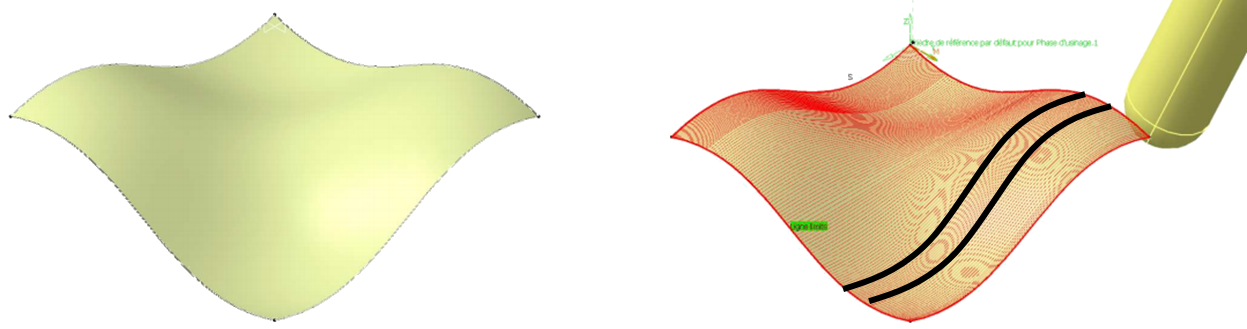
\includegraphics[width=.8\textwidth]{images/surf.png}
 
\textit{Courbes et surfaces obtenues en utilisant des logiciels de CAO }
\end{center}


Les courbes de Bézier sont des courbes paramétriques définies par $n$ points $P_i$ de coordonnées $\left(x_i,y_i\right)$ appelés pôles. Ainsi, les coordonnées d'un point $M(u)=\left(x(u),y(u)\right)$ appartenant à la courbe sont définies par : 

\begin{minipage}[c]{.45\linewidth}

$$
\forall u \in [0,1] \quad 
\left\{
\begin{array}{l}
x(u)=\sum\limits_{i=0}^{n}B_i^n(u)x_i\\
y(u)=\sum\limits_{i=0}^{n}B_i^n(u)y_i
\end{array}
\right.
$$
Avec :
$$
B_i^n(u)=\left(
\begin{array}{c}
n\\
i
\end{array}\right)u^i\left(1-u \right)^{n-i}
\text{, }
\left(
\begin{array}{c}
n\\
i
\end{array}\right)=\dfrac{n!}{i!(n-i)!}$$
$$
 \forall n\in\mathbb{N^*}, n!=\prod\limits_{i=1}^{n}i \text{ et } 0!=1
 $$


\end{minipage} \hfill
\begin{minipage}[c]{.45\linewidth}
\begin{center}
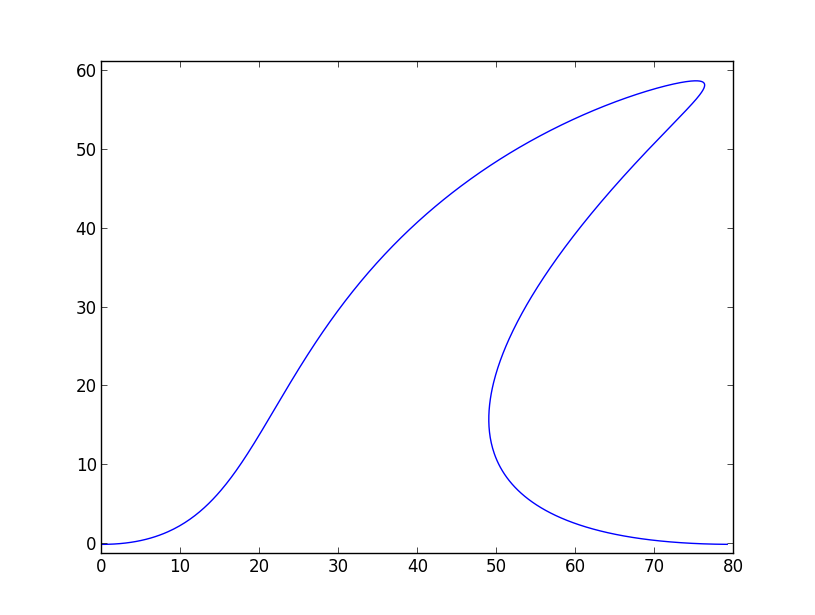
\includegraphics[width=.9\textwidth]{images/shark.png}
\textit{Tracé d'une courbe de Bézier}
\end{center}
\end{minipage}

\vspace{.5cm}


%\begin{center}
%\includegraphics[width=.9\textwidth]{png/cyclev.png}

%\textit{Cycle de conception d'un produit}
%\end{center}

Le tracé de ces courbes fait appel à la définition de fonctions, de boucles, d'instructions conditionnelles qui sont au c\oe{}ur du développement de programmes informatiques. 

Le but de ce cours est de définir les instructions de base qui doivent permettre la réalisation d'algorithmes. 


\begin{prob}
\textsc{Problématique :}

Connaissant la définition mathématique d'une courbe de Bézier, quels sont les algorithmes qui permettent de tracer une telle courbe ?
\end{prob}


\begin{comp}
Vous devrez être capables d'\textbf{imaginer} et \textbf{concevoir} une solution algorithmique modulaire, utilisant des méthodes de programmation, des structures de données appropriées pour le problème étudié :
\begin{itemize}
\item \textit{Alg -- C1 :} comprendre un algorithme et expliquer ce qu’il fait;
\item \textit{Alg -- C3 :} concevoir un algorithme répondant à un problème précisément posé;
\item \textit{Alg -- C4 :} expliquer le fonctionnement d’un algorithme;
\item \textit{Alg -- C5 :} écrire des instructions conditionnelles avec alternatives, éventuellement imbriquées.
\end{itemize}
\end{comp}
 

\setlength{\parskip}{0ex plus 0.2ex minus 0ex}
 \renewcommand{\contentsname}{}
 \renewcommand{\baselinestretch}{1}

\tableofcontents

 \renewcommand{\baselinestretch}{1.2}
\setlength{\parskip}{2ex plus 0.5ex minus 0.2ex}

% \vspace{1cm}
\textit{Ce document évolue. Merci de signaler toutes erreurs ou coquilles.}


\section{Quelques rudiments}

\subsection{Algorithmes et programmes \cite{wack}}
\begin{defi}
\textbf{Algorithmes}

Un algorithme est une procédure permettant de résoudre un problème, écrite de façon
suffisamment détaillée pour pouvoir être suivie sans posséder de compétence particulière
ni même comprendre le problème que l’on est en train de résoudre.
\end{defi}

\begin{defi}
\textbf{Programme}

Un programme est la traduction d’un algorithme dans un langage particulier,
à la fois interprétable par la machine et compréhensible par l’homme. Il est constitué
d’un assemblage d’instructions, regroupées dans un fichier texte appelé le code source du
programme.
\end{defi}

\begin{warn}
En toutes circonstances, il faudra s'assurer que : 
\begin{itemize}
\item le résultat de l'algorithme est conforme au résultat attendu;
\item l'algorithme soit documenté. 
\end{itemize}
\end{warn}

\begin{exemple}

\textit{On demande de réaliser le calcul de $n!$. Un programmeur propose le code suivant. Le programme répond-il au cahier des charges ?}


\begin{minipage}[c]{.35\linewidth}
\begin{py}
\begin{python}
n=input("Saisir un nombre : ")
n=int(n)
res=0
for i in range(1,n):
    res = res*n
print(res)
\end{python}
\end{py}
\end{minipage} \hfill
\begin{minipage}[c]{.62\linewidth}
\end{minipage}
\end{exemple}

\subsection{Sémantique}

\begin{defi}
\textbf{Opérateurs}

Chaque type de donnée admet un jeu d’opérateurs adaptés :
\begin{itemize}
\item opérateurs arithmétiques : $+,\; -,\; *,\; /,\; \text{div},\; \text{mod},\; \hat\quad,\; **$;
\item opérateurs relationnels : $==,\; \neq,\; >,\;<,\; \leq,\; \geq$;
\item opérateurs logiques : négation, ou, et;
\item opérateur d'affectation : $\leftarrow$.
\end{itemize}
\end{defi}


\begin{defi}
\textbf{Expressions -- Instructions}

Une expression est un groupe de nombres, constantes, variables liées par des opérateurs. Elles sont évaluées pour donner un résultat. 

Une séquence d'instructions est appelé bloc d'instructions. Lors de l'exécution du programme, les instructions s'exécutent les unes après les autres.
\end{defi}





\begin{exemple}

\begin{minipage}[c]{.47\linewidth}
Le pseudo-code (ou pseudo langage) est une représentation non normalisée d'un algorithme ou d'une fonction. Il permet d'écrire un algorithme en utilisant le langage naturel. 
\end{minipage}\hfill
\begin{minipage}[c]{.45\linewidth}
\begin{pseudo}
\begin{algorithm}[H]
\Fonction{
Instruction 1\\
...\\
Instruction 2\\
}
\end{algorithm}
\end{pseudo}
\end{minipage}

\vspace{.25cm}

\begin{minipage}[c]{.47\linewidth}
En python, les instructions peuvent être séparées par des retours à la ligne, des points-virgules. Dans le cas des blocs d'instructions, les instructions sont \textbf{indentées} (4 espaces). 

\end{minipage}\hfill
\begin{minipage}[c]{.47\linewidth}
\begin{py}
\begin{minipage}{.9\linewidth}
\begin{python}[showspaces=true]
Instruction1
Instruction2
Instruction1;Instruction2
Bloc : 
    Instruction 1
    Instruction 2
\end{python}
\end{minipage}
\end{py}
\end{minipage}


\begin{minipage}[c]{.47\linewidth}
En Scilab : une virgule, un point virgule, un retour à la ligne peuvent séparer des instructions. (Lorsque les instructions sont terminées par un point virgule, les résultats des instructions ne sont pas affichées à l'écran.)

Les blocs sont terminés par \textsf{end}.
\end{minipage}\hfill
\begin{minipage}[c]{.47\linewidth}
\begin{sci}
\begin{scilab}
Instruction1
Instruction2
Instruction1,Instruction2
Instruction1;Instruction2;
Debut Bloc
Instruction 1
Instruction 2
end
\end{scilab}
\end{sci}
\end{minipage}


\end{exemple}


\subsection{Définition de fonctions}
\subsubsection{Les fonctions}
\begin{defi}
\textbf{Définitions}

Les fonctions permettent :
\begin{itemize}
\item d’automatiser des tâches répétitives;
\item d’ajouter de la clarté à un algorithme;
\item d’utiliser des portions de code dans un autre algorithme.
\end{itemize}
\end{defi}
Lors de l'exécution d'un programme, il est très courant qu'une même séquence d'instruction soit répété un grand nombre de fois. Ainsi, il est courant de décomposer un problème sous forme de plusieurs sous programmes élémentaires. 

%\begin{defi}

%\end{defi}


\begin{exemple}
\textit{Courbes de Bézier d'ordre 2}

Prenons le cas où nous souhaitons connaître les coordonnées d'un point appartenant à une courbe de Bézier définie par 3 points. 
Dans ce cas,
$$
\forall u \in [0,1] \quad 
\left\{
\begin{array}{l}
x(u)= \left(1-u\right)^2 x_0 + 2u\left(1-u\right)x_1 + u^2 x_2\\
y(u)= \left(1-u\right)^2 y_0 + 2u\left(1-u\right)y_1 + u^2 y_2
\end{array}
\right.
$$

Écrivons la fonction permettant d'évaluer une coordonnée en un paramètre donné. Autrement dit :
$$
\forall u \in[0,1] f(u)= \left(1-u\right)^2 x_0 + 2u\left(1-u\right)x_1 + u^2 x_2
$$


\begin{pseudo}
\begin{algorithm}[H]
\Donnees{u,$x_0$,$x_1$,$x_2$}

\Fonction{
Fonction $f(u,x_0,x_1,x_2)$:\\
$val \gets (1-u)^2x_0 + 2u(1-u)x_1 + u^2x_2$\\
\Retour{val}
}
print $f(0.5,0,1,2)$  
\end{algorithm}
\end{pseudo}



\begin{minipage}[c]{.48\linewidth}
\begin{py}
\begin{python}
def f(u,x0,x1,x2):
    val = (1-u)**2*x0 + 2*u*(1-u)*x1 + u**2*x2
    return val

print(f(0.5,0,1,2))    
\end{python}
\end{py}
\end{minipage}\hfill
\begin{minipage}[c]{.48\linewidth}
\begin{sci}
\begin{scilab}
function [val]=f(u,x0,x1,x2)
  val=(1-u)**2*x0+2*u*(1-u)*x1+u**2*x2;
endfunction

printf("%f",f(0.5,0,1,2))
\end{scilab}
\end{sci}
\end{minipage}

Dans ce cas, rien ne permet de contrôler que $u$ appartient bien à l'intervalle 
$[0,1]$ et que les arguments $x0$, $x1$, et $x2$, sont bien des nombres réels.
\end{exemple}


\subsubsection{Variables locales -- Variables globales}
\begin{defi}
\textbf{Visibilité :} Une variable globale est définie en dehors de toute fonction, une variable locale est définie dans une fonction et masque toute autre variable portant le même nom.

\textbf{Durée de vie :} Une variable globale existe durant l'exécution du programme, une variable locale existe durant l'exécution de la fonction.

\textbf{Par défaut, dans un langage interprété, les variables sont locales à un bloc.}
\end{defi}


\begin{exemple}

\textit{Comportement de Python lors de l'utilisation de variables}

\begin{minipage}[t]{.2\linewidth}
\begin{py}
\begin{python}
def f(x):
    a=3
    b=2
    res = a*x+b
    return res
a=4
b=f(a)
\end{python}
\end{py}
\end{minipage} \hfill
\begin{minipage}[t]{.78\linewidth}
Quel est le but de la fonction $f$ ? Que se passe-t-il à l'écran si elle est exécutée ? Après exécution du programme, que valent $a$, $b$ et $x$ ?
\end{minipage}

\vspace{2cm}

\begin{minipage}[t]{.2\linewidth}
\begin{py}
\begin{python}
def f(x):
    x=x+2
    return x
x=4
y=f(x)
\end{python}
\end{py}
\end{minipage} \hfill
\begin{minipage}[t]{.78\linewidth}
Quel est le but de la fonction $f$ ? Que se passe-t-il à l'écran si elle est exécutée ? Après exécution du programme, que valent $x$ et $y$ ?
\end{minipage}

\begin{minipage}[t]{.2\linewidth}
\begin{py}
\begin{python}
def f(x):
    x[0]=0
    return x
x=[1,2,3]
y=f(x)
\end{python}
\end{py}
\end{minipage} \hfill
\begin{minipage}[t]{.78\linewidth}
Quel est le but de la fonction $f$ ? Que se passe-t-il à l'écran si elle est exécutée ? Après exécution du programme, que valent $x$ et $y$ ?
\end{minipage}

\end{exemple}


\begin{exemple}
\textit{Exemples de variables globales -- Courbes de Bézier d'ordre 2}

On reprend le cas précédent. On se place dans le cas où le programme n'utilise que des courbes Bézier d'ordre 2 et où les pôles restent inchangés. On souhaite alors définir la fonction $f$ sans avoir à rappeler les coordonnées de chacun des pôles.

 

\begin{pseudo}
\begin{algorithm}[H]
\Donnees{u}
\Donnees{Global : $x_0\gets 0$,$x_1\gets 1$,$x_2\gets 2$}
\Fonction{
Fonction $f(u)$:\\
$val \gets (1-u)^2x_0 + 2u(1-u)x_1 + u^2x_2$\\
\Retour{val}
}
print $f(0.5)$
\end{algorithm}
\end{pseudo}

\begin{minipage}[c]{.48\linewidth}
\begin{py}
\begin{python}
def fx(u):
    val = (1-u)**2*x0 + 2*u*(1-u)*x1 + u**2*x2
    return val
    
global x0,x1,x2
x0,x1,x2=0,1,2

print(fx(0.5))  
\end{python}
\end{py}
\end{minipage}\hfill
\begin{minipage}[c]{.48\linewidth}
\begin{sci}
\begin{scilab}
function [val]=f(u)
  val=(1-u)**2*x0+2*u*(1-u)*x1+u**2*x2;
endfunction

global x0 x1 x2
x0=0;x1=1;x2=2;

printf("%f",f(0.5))
\end{scilab}
\end{sci}
\end{minipage}
\end{exemple}

\begin{rem}
De manière générale, on essaiera d'utiliser le moins possible les variables globales.
\end{rem}

%\subsubsection{Attributs d'un objet}

%Visibilité des attributs d'un objet : publique, protégée et privée selon la définition de l'objet.

\subsubsection{Documentation des fonctions}
En programmation, il est indispensable de documenter les fonctions. En effet, il n'est pas toujours facile de se replonger dans un algorithme qu'on a écrit et il est indispensable de le ponctuer de commentaires pour pouvoir bien comprendre le but d'une fonction, d'une boucle \textit{etc}.


\begin{py}
En python un commentaire court commence par le signe \#. Les commentaires longs sont encadrés par trois guillemets ".

\begin{python}
# ======= Debut de la definition des fonctions =======
def f(u,x0,x1,x2):
    """
    Retourne la coordonnee d'un point pour une courbe de Bezier d'ordre 2
    Keyword arguments:
    u -- parametre de la courbe parametree (doit etre compris entre 0 et 1)
    x0 -- coordonnee du pole 0 (sur x, y ou z)
    x1 -- coordonnee du pole 1 (sur x, y ou z)
    x2 -- coordonnee du pole 2 (sur x, y ou z)
    """
    val = (1-u)**2*x0 + 2*u*(1-u)*x1 + u**2*x2
    return val
# ======= Fin de la definition des fonctions =======
\end{python}

Lorsqu'une fonction est commentée comme dans l'exemple ci-dessus, on peut accéder à de la documentation sur la fonction en procédant ainsi :
\begin{python}
>>> help(f)
>>> f.__doc__
\end{python}

Enfin, sous linux, il est possible de générer automatiquement de la documentation au format \textsf{html} :

\textsf{pydoc -w ./ExempleCours.py} 
\end{py}

\begin{sci}

En scilab un commentaire commence par un double slash : //. 

\begin{scilab}
// La fonction f etourne la coordonnee d'un point pour une courbe de Bezier d'ordre 2
//     * u : parametre 
//     * x0, x1, x2 coordonnees des poles 0 1 et 2
function [val]=f(u,x0,x1,x2)
  val=(1-u)**2*x0+2*u*(1-u)*x1+u**2*x2;
endfunction
\end{scilab}
\end{sci}

\subsection{Import de méthodes et de fonctions}

Par défaut, Python ne permet que de réaliser des opérations élémentaires (opérations mathématiques élémentaires, comparaisons, boucles \textit{etc.}). 

Il existe par ailleurs un grand nombre de bibliothèques permettant par exemple de manipuler des fonctions mathématiques ($\sin$, $\cos$, $\sqrt{\;}$ \textit{etc.}), des bibliothèques permettant de tracer des courbes, des bibliothèques permettant d'interroger des bases de données \textit{etc.}

 

Pour utiliser les méthodes liées à ces bibliothèques, on procèdera ainsi :

\begin{py}
\begin{python}
import math  # Import de toutes les methodes de la bibliotheque math
math.sqrt(2) # Permet d'utiliser la methode sqrt de la bibliotheque math
from math import sqrt # Import de la methode sqrt de la bibliotheque math

import os # Import de la bibliotheque os permettant de realiser des operations systemes
\end{python}
\end{py} 

\begin{warn}
Il est déconseillé d'utiliser la méthode d'import suivante : 
\begin{python}
from os import *
\end{python}

En effet, si des méthodes ont le même nom, seules les méthodes de la dernière bibliothèque appelée ou de la dernière fonction nommée sont utilisables. 
\end{warn}


\begin{exemple}
\textit{Fonction pow : Calcul de $x^\alpha$.}

\end{exemple}
\section{Instructions conditionnelles}



\subsection{Expressions booléennes}
\begin{defi}
Une expression booléenne est une instruction qui renvoie la valeur "vrai" ou "faux".
\end{defi}

\begin{defi}
\textbf{Opérateurs de comparaison}


\begin{minipage}[c]{.3\linewidth}

\begin{pseudo}
\begin{algorithm}[H]
$2=8 $ \\
$2\neq8 $\\
$2\geq 8 $\\
$2>8 $\\
$2\leq 8$\\
$2<8$\\
\end{algorithm}
\end{pseudo}

\end{minipage} \hfill
\begin{minipage}[c]{.3\linewidth}
\begin{py}
\begin{python}
 >>> 2==8
	False
 >>> 2!=8
	True
 >>> 2>=8
	False
 >>> 2>8
	False
 >>> 2<=8
	True
 >>> 2<8
	True
\end{python}
\end{py}
\end{minipage} \hfill
\begin{minipage}[c]{.3\linewidth}
\begin{sci}
\begin{scilab}
 --> 2==8
	F
 --> 2!=8
	T
 --> 2>=8
	F
 --> 2>8
	F
 --> 2<=8
	T
 --> 2<8
	T
\end{scilab}
\end{sci}
\end{minipage}

\end{defi}



\subsection{Boucle \textsl{Tant que}}

\begin{defi}
La boucle \textsf{Tant que} appelée aussi boucle \textsf{while} permet de répéter une instruction tant qu'une condition reste vraie.
\end{defi}

\begin{rem}
Les boucles ont la plupart du temps besoin d'être incrémentées. Pour cela plusieurs solutions sont possibles.

\begin{minipage}[c]{.3\linewidth}
\begin{pseudo}
\begin{algorithm}[H]
$i \gets 1$\\
$i \gets i+1$\\
\end{algorithm}
\end{pseudo}
\end{minipage} \hfill
\begin{minipage}[c]{.3\linewidth}
\begin{py}
\begin{python}
>>> i=1
>>> i=i+1;print(i)
    2
>>> i+=1;print(i)
    3
>>> i+=2;print(i)
    5
\end{python}
\end{py}
\end{minipage} \hfill
\begin{minipage}[c]{.3\linewidth}
\begin{sci}
\begin{scilab}
--> i=1;
--> i=i+1;
\end{scilab}
\end{sci}
\end{minipage} 

\end{rem}


\begin{exemple}
\textit{Implémentation de la fonction "factorielle"}

On peut définir la fonction factorielle ainsi : 
$$
\forall  n\in \mathbb{N}
\left\{
\begin{array}{l}
\text{si } n=0 \quad n!=1\\
\text{sinon } n !=\prod\limits_{i=1}^n i
\end{array}
\right.
$$
 
On s'intéresse à la programmation du cas où $n$ est supérieur ou égal à 1.

\begin{minipage}[c]{.3\linewidth}
\begin{pseudo}
\begin{algorithm}[H]
\Fonction{
factorielle($n$):\\
$i\gets1$\\
$res\gets1$\\
\Tq{$i\leq n$}{
$res \gets res \cdot i$ \\
$i\gets i+1$}
\Retour{res}
}
\end{algorithm}
\end{pseudo}
\end{minipage}\hfill
\begin{minipage}[c]{.3\linewidth}
\begin{py}
\begin{python}
def factorielle(n):
        i=1    
        res=1
        while i<=n:
            res=res*i
            i+=1
        return res
\end{python}
\end{py}
\end{minipage}\hfill
\begin{minipage}[c]{.3\linewidth}
\begin{sci}
\begin{scilab}
function [res]=factorielle(n)
  i=1;
  res=1;
  while i<=n
    res = res*i
    i=i+1
  end
endfunction
\end{scilab}
\end{sci}
\end{minipage}

\end{exemple}



\begin{warn}
Lors de la réalisation d'une boucle \textsl{while} il faut veiller à ce que l'instruction conditionnelle change d'état afin de sortir de la boucle et de ne pas provoquer une boucle sans fin...
\end{warn}


\subsection{Instruction \textsl{Si, Sinon}}

\begin{defi}
La boucle \textsf{Si} appelée aussi boucle \textsf{if} permet d'exécuter une instruction si une condition est vraie.
\end{defi}


\begin{exemple}
\textit{Implémentation de la fonction "factorielle"}

On souhaite maintenant gérer le cas où $n=0$. Dans ce cas, le calcul de $n!$ est différent du cas où $n>0$.

\begin{minipage}[c]{.35\linewidth}
\begin{pseudo}
\begin{algorithm}[H]
\Fonction{
factorielle($n$):\\
\eSi{n=0}{
\Retour{1}
}{
$i\gets1$\\
$res\gets1$\\
\Tq{$i\leq n$}{
$res \gets res \cdot i$ \\
$i\gets i+1$}
\Retour{res}
}}
\end{algorithm}
\end{pseudo}
\end{minipage}\hfill
\begin{minipage}[c]{.3\linewidth}
\begin{py}
\begin{python}
def factorielle(n):
    if n==0:
        return 1
    else :
        i=1    
        res=1
        while i<=n:
            res=res*i
            i+=1
        return res
\end{python}
\end{py}
\end{minipage}\hfill
\begin{minipage}[c]{.3\linewidth}
\begin{sci}
\begin{scilab}
function [res]=factorielle(n)
  if n==0
    res =1;
  else
    i=1;
    res=1;
    while i<=n
      res = res*i
      i=i+1
    end
  end  
endfunction
\end{scilab}
\end{sci}
\end{minipage}

\textit{Remarque :} Il faudrait vérifier que $n$ est bien un \textbf{entier} \textbf{positif ou nul}.
\end{exemple}


\begin{exemple}
\textit{Implémentation de la fonction "factorielle"}

On souhaite maintenant s'assurer que $n$ est bien un \textbf{entier} \textbf{positif ou nul}.


%\begin{pseudo}
%En pseudo-code
%\end{pseudo}

\begin{py}
\begin{python}
def calc_factorielle(n):
    if (type(n)==int) & (n>=0):
        return factorielle(n) 
    else :
        print("Oooops... il faut saisir un nombre entier POSITIF ou nul")
\end{python}
\end{py}

%\begin{sci}
%\begin{scilab}
%Scilab
%\end{scilab}
%\end{sci}

\textit{Remarque :} Il faudrait vérifier que $n$ est du bon type.
\end{exemple}


\subsubsection*{La gestion des erreurs}


\begin{exemple}
\textit{Implémentation de la fonction "factorielle"}

On souhaite maintenant s'assurer que $n$ est du bon type.

%\begin{pseudo}
%E pseudo-code
%\end{pseudo}

\begin{py}
\begin{python}[moreemph={[4], 46, 48}]
def calc_factorielle(n):
    try:
        if (type(n)==int) & (n>=0):
            return(factorielle(n))
        else :
            print("Oooops... il faut saisir un nombre entier POSITIF ou nul")
    except TypeError:
        print("Oooops... le type de la variable n'est pas le bon")
\end{python}
\end{py}

%\begin{sci}
%\begin{scilab}
%Scilab
%\end{scilab}
%\end{sci}

\end{exemple}


\begin{rem}
Pour aller plus loin : on peut définir ses propres exceptions et gérer les messages d'erreur. 
\begin{py}
\begin{python}
class MonException(Exception):
    def __init__(self,raison):
        self.raison = raison
     
    def __str__(self):
        return self.raison
 
def calc_factorielle(n):
    if n > 20:
        raise MonException("Il faut saisir un entier positif ou nul")
    else:
        return factorielle(n)
\end{python}
\end{py}
\end{rem}



%\begin{itemize}
%\item Expressions booléennes et opérateurs logiques simples.
%\item Sémantique (fond)
%\item Syntaxe (forme) : instructions 	
%\begin{itemize}
%\item si, sinon (pseudo langage)
%\item if, elif, else (python)
%\item if, then, else, elseif, select, case, end (scilab)
%\end{itemize}
%\item Problème d’une comparaison avec un nombre réel. Le type float est le plus souvent une %approximation
%\end{itemize}



\section{Instructions itératives}

\begin{defi}
Une instruction itérative permet de répéter une suite d'instructions un nombre déterminé de fois. 
On parle aussi de boucle \textsf{for}.
\end{defi}

%\begin{rem}
%Incréments range...
%\end{rem}

\begin{exemple}
\textit{Courbes de Bézier d'ordre 2}

Nous avons précédemment étudié la fonction permettant de calculer l'abscisse ou l'ordonnée d'un point d'une courbe de Bézier. 

Pour afficher une telle courbe une solution consiste en calculer les coordonnées d'un nombre $n$ de points et de relier ces points par des segments de droite. Plus le nombre de points sera élevé plus la courbe paraîtra lisse, mais le temps de calcul sera d'autant plus élevé. On rappelle qu'une courbe de Bézier est une courbe paramétrique définie pour $u\in[0;1]$ et que la fonction $f$ est définie par $f(u)=\left(1-u\right)^2x_0 + 2u\left(1-u\right)x_1+u^2x_2$.

Il va falloir \textbf{discrétiser} l'intervalle $[1,0]$.

\begin{minipage}[c]{.36\linewidth}
\begin{pseudo}
\begin{algorithm}[H]
Tableau $x$;\\
Tableau $y$;\\
$x_0 \gets 0$; $y_0 \gets 0$\\
$x_1 \gets 10$; $y_1 \gets 10$\\
$x_2 \gets 20$; $y_2 \gets 0$\\
$i \gets 0$; $n \gets 50$\\
\Pour{i de 0 à $n$}{
$u \gets i/(n-1)$\\
$ x[i] \gets f(u,x_0,x_1,x_2)$\\
$ y[i] \gets f(u,y_0,y_1,y_2)$\\
$i \gets i+1$\\
}
Afficher($x$,$y$)
\end{algorithm}
\end{pseudo}
\end{minipage}\hfill
\begin{minipage}[c]{.3\linewidth}
\begin{py}
\begin{python}
import numpy as np
import pylab as pl

x0=0;y0=0
x1=10;y1=10
x2=20;y2=0
n=50
x,y=[],[]
for i in range(0,n):
    u=i/(n-1)
    x.append(f(u,x0,x1,x2))
    y.append(f(u,y0,y1,y2))
pl.plot(x,y)
pl.axis('equal')
pl.show()
\end{python}
\end{py}
\end{minipage}\hfill
\begin{minipage}[c]{.3\linewidth}
\begin{sci}
\begin{scilab}
x0=0;y0=0;
x1=10;y1=10;
x2=20;y2=0;
n=50;
for i=1:n
  u=i/n;
  x(i)=f(u,x0,x1,x2);
  y(i)=f(u,y0,y1,y2);
end
plot2d(x,y) // a verifier
\end{scilab}
\end{sci}
\end{minipage}



\begin{minipage}[c]{.22\linewidth}
\begin{center}
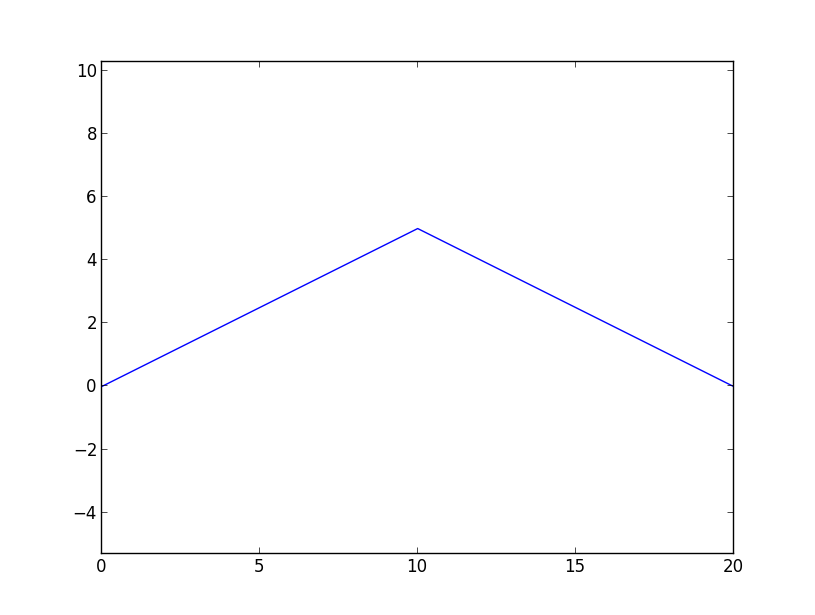
\includegraphics[width=\textwidth]{images/n3}

$n=3$
\end{center}
\end{minipage}\hfill
\begin{minipage}[c]{.22\linewidth}
\begin{center}
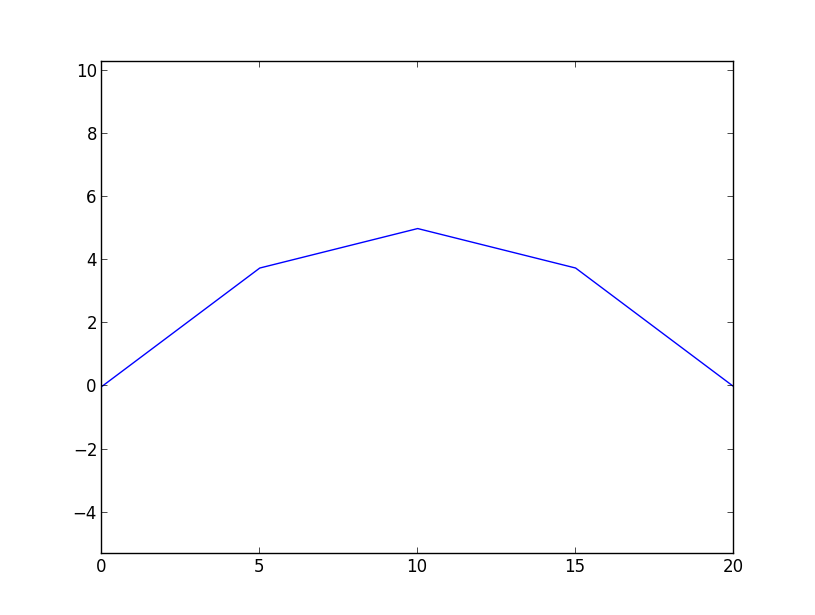
\includegraphics[width=\textwidth]{images/n5}

$n=5$
\end{center}
\end{minipage}\hfill
\begin{minipage}[c]{.22\linewidth}
\begin{center}
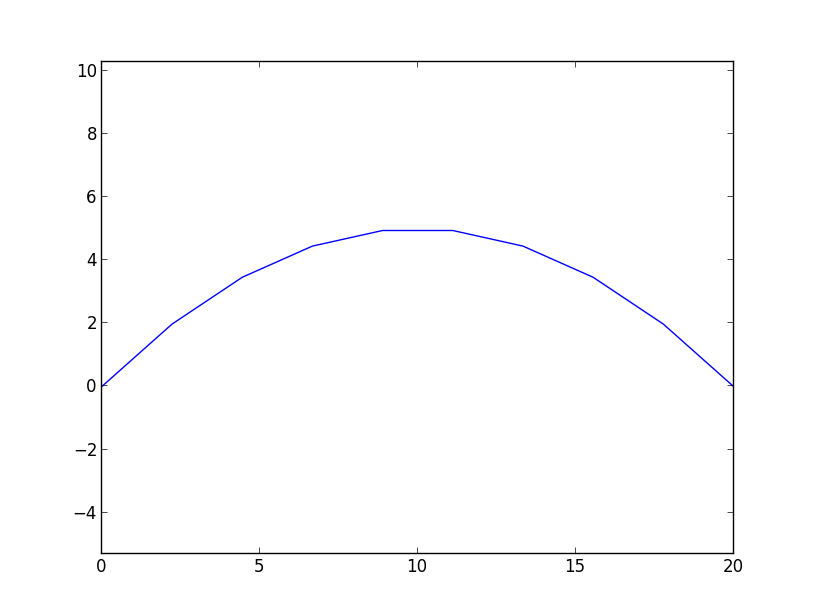
\includegraphics[width=\textwidth]{images/n10}

$n=10$
\end{center}
\end{minipage}\hfill
\begin{minipage}[c]{.22\linewidth}
\begin{center}
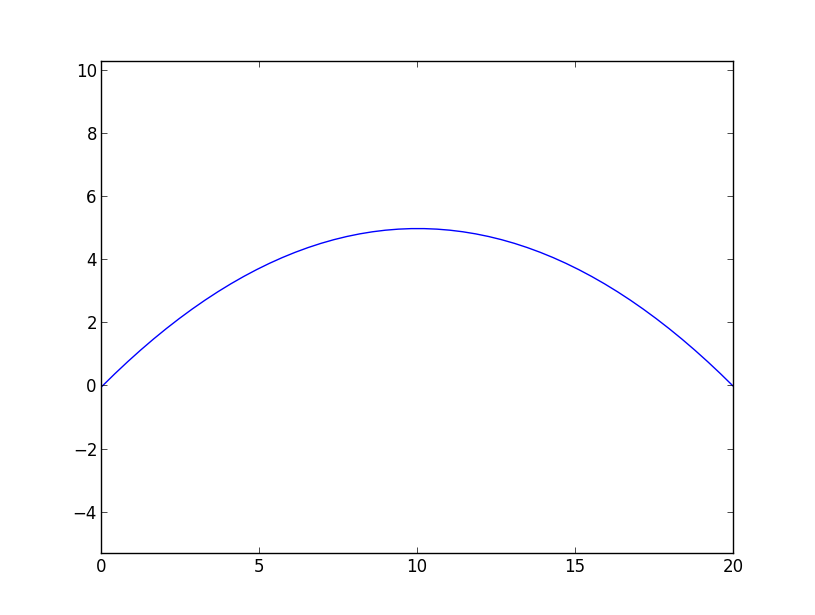
\includegraphics[width=\textwidth]{images/n50}

$n=50$
\end{center}
\end{minipage}
\end{exemple}


\begin{rem}
En python, \textsf{range} permet de définir la liste des valeurs qui vont être utilisées lors du parcours de la boucle \textsf{for}.  Cette fonction peut prendre jusqu'à 3 arguments : le premier argument désigne la valeur de départ, le second la valeur de fin (exclue), la troisième la valeur de l'incrément. 
\end{rem}

\begin{rem}
La boucle \textsf{while} définie précédemment est aussi une instruction itérative. 
\end{rem}


\begin{exemple}
\textit{Courbes de Bézier d'ordre 2}


\begin{minipage}[c]{.49\linewidth}
\begin{py}
\begin{python}
inc = 0.1
while u<=1 :
    x.append(f(u,x0,x1,x2))
    y.append(f(u,y0,y1,y2))
    u += inc
\end{python}
\end{py}
\end{minipage}\hfill
\begin{minipage}[c]{.49\linewidth}
\begin{sci}
\begin{scilab}
inc = 0.1; i = 1;
u=0;
x = []; y = [];
while u<=1
    x(i)=f(u,x0,x1,x2);
    y(i)=f(u,y0,y1,y2);
    u=u+inc;
    i=i+1;
end
\end{scilab}
\end{sci}
\end{minipage}

\end{exemple}



\begin{exemple}
\textit{\`A partir des fonctions précédentes et de la définition mathématique d'une courbe de Bézier, donner la structure d'un programme permettant de tracer une courbe de Bézier à partir d'une liste de pôles.}

\end{exemple}
\begin{thebibliography}{2}
\bibitem{wack}{\textit{Wack, Conchon, Courant, de Falco, Dowek, Filliatre, Gonnord}, Informatique pour tous en classes préparatoires aux grandes écoles, Éditions Eyrolles.}
\bibitem{pb}{\textit{Patrick Beynet}, Cours d'informatique en CPGE, Lycée Rouvière Toulon, UPSTI.}
\end{thebibliography}




\end{document}


